\documentclass[11pt]{article}

\usepackage[margin=1in]{geometry}
\usepackage[T1]{fontenc}
\usepackage{amsmath}
\usepackage{booktabs}
\usepackage{graphicx}
\usepackage{hyperref}
\hypersetup{hidelinks}
\setlength{\emergencystretch}{2em}

\title{11-768 HW2: Evaluating a Data-Visualization Agent}
\author{Yubo Chen\\Andrew ID: \texttt{yuboc}}
\date{}

\begin{document}
\maketitle

\begin{quote}
\small
\textbf{Final experiment summary.}
Parts 1--2 below record the completed baseline experiment, two evidence-backed
error analyses, both proposed implementations, and the full seed-set comparison.
Part 3 task design, all 15 fixed-agent runs, and pre-iteration authored
evaluation are complete. AI-assisted reference annotations were reviewed
and confirmed by the author for all 15 runs. The author ran initialization,
structural validation, and scoring.
The Harbor worked example and all five authored package experiments are
complete: each reference solution scored 1.0, and the two authored mutants
scored 0.0 and 1.0.
Part 4's additional validator improvement is implemented and documented below;
the selected final source has complete 110-run seed and 15-run authored
evaluations. The author ran both final scoring commands, obtaining
macro-MCC $0.4462$ on seed runs and $0.5000$ on authored runs.
The author also ran the complete Docker-backed submission check; it
reported \texttt{submission valid}, with all five oracle rewards 1.0
and the two mutant rewards 0.0 and 1.0.
\end{quote}

The four reproduced seed figures are unchanged copies in
\path{report_assets/}; the authored shared-axis figure is loaded directly
from the required \path{runs/} directory. These source-image directories
must accompany the source to recompile the report; the PDF embeds the images.

\section{Part 1: Examine Seed Agent Runs}

\subsection{Comparison of Ground-Truth and Validator Labels}
\label{sec:baseline}

\paragraph{Evaluation target and evidence.}
The object being evaluated is the validator's ability to diagnose an existing
visualization-agent run, not its ability to generate a new plot.
The released \path{artifacts/<run_id>/result.json} files contain the task,
input-file references, and agent trajectories; the corresponding
\path{figure.png}, when present, is the final rendered artifact.
The provided \path{seed_labels.json} supplies the human labels used for
evaluation. The baseline's predictions are stored separately in
\path{output/baseline_predictions.json}. All comparisons are keyed by
\texttt{run\_id}, rather than relying on \texttt{task\_id} being unique.

\paragraph{Baseline and serving configuration.}
The experiment used the supplied, unmodified \path{validator/baseline.py}
and the fixed judge model
\path{Qwen/Qwen3-VL-30B-A3B-Instruct-FP8}, served under the alias
\texttt{validator} by \path{infrastructure/validator_model.py}.
The supplied deployment uses one L40S GPU, a maximum of one serving container,
and a 32,768-token maximum model context. The validator client uses
temperature zero; each baseline judgment requests at most 250 output tokens.
No alternative judge model was used.

For each run, the baseline first asks about execution failure. If that check
returns an error, it stops evaluating the run. Otherwise, it separately asks
about data correctness, chart design, and readability. Each question includes
the task, serialized trajectory, input-file contents, and the figure if one
exists. The installed baseline attempts full evidence first. On a recognized
context-overflow error, its implementation compacts trajectory and input text
and, if necessary, repeatedly downscales the image. This description follows
the actual released implementation, rather than assuming that every request
retains the original image resolution. The prediction file does not preserve
the exact request used on each attempt, so I do not attribute any particular
case below to truncation or downscaling.

\paragraph{Reproduction commands and coverage.}
The baseline was run and then scored using:
\begin{verbatim}
uv run python -m validator.runner \
  --solution validator.baseline \
  --artifacts artifacts \
  --out output/baseline_predictions.json

uv run python -m workflow score \
  --labels seed_labels.json \
  --predictions output/baseline_predictions.json
\end{verbatim}
The saved predictions cover all 110 released runs, with 110 unique run IDs,
no missing IDs, no unexpected IDs, and no duplicate entries.
Scoring requires matching label and prediction coverage; the results below
are not scores on an incomplete subset.

\paragraph{Scoring convention.}
Each error family is a separate binary classification problem. Here TP means
correctly reporting an error of that family; TN means correctly not reporting
it; FP is a false alarm; and FN is a missed error. A TN for one family does not
imply that the run is free of errors in other families.
The Matthews correlation coefficient is
\[
 \mathrm{MCC}
 =
 \frac{TP\cdot TN-FP\cdot FN}
 {\sqrt{(TP+FP)(TP+FN)(TN+FP)(TN+FN)}}.
\]
The scorer reports zero when the denominator is zero.
The macro-MCC is the unweighted average of the four family MCCs, calculated
from their unrounded values; it is not an accuracy percentage.

There are 12 human-labeled execution failures. These runs are excluded from
the other three families' confusion counts, as required by the assignment.
Consequently, execution failure is scored on 110 runs and the other families
on 98. A \emph{predicted} execution failure does not receive this exemption.
Every family has both positive and negative ground-truth support in this set.

\begin{table}[htbp]
\centering
\small
\begin{tabular}{lrrrrrr}
\toprule
Error family & Scored runs & TP & TN & FP & FN & MCC \\
\midrule
\texttt{execution\_failure} & 110 & 4 & 65 & 33 & 8 & $-0.0022$ \\
\texttt{wrong\_data}        & 98  & 0 & 73 & 0  & 25 & $0.0000$ \\
\texttt{wrong\_chart}       & 98  & 3 & 27 & 0  & 68 & $0.1096$ \\
\texttt{hard\_to\_read}     & 98  & 0 & 59 & 0  & 39 & $0.0000$ \\
\bottomrule
\end{tabular}
\caption{Measured baseline results against the released human labels.
Macro-MCC is \textbf{0.0268}. Values are rounded to four decimal places.}
\label{tab:baseline}
\end{table}

\paragraph{Where disagreements concentrate.}
The baseline over-reports execution failure: it reports this family on
37 runs, of which only four are true positives and 33 are false positives.
It also misses eight of the 12 actual execution failures. This yields an
execution MCC very close to zero.
On the 98 runs eligible for the remaining families, it detects none of the
25 data errors or 39 readability errors, and only three of 71 chart-design
errors. The zero MCCs for data and readability reflect constant negative
predictions, not zero accuracy: their TN counts are nonzero, but none of
their positive examples are detected.

The execution-first control flow contributes to downstream omissions:
among the 33 falsely predicted execution failures, the human labels contain
three \texttt{wrong\_data} positives, 14 \texttt{wrong\_chart} positives,
and eight \texttt{hard\_to\_read} positives. These counts overlap across runs
and must not be summed as a number of distinct runs.
They also do not explain all downstream false negatives. In particular,
the second error type below occurs on runs that were not stopped by the
execution check.

\paragraph{Case-analysis method and limitations.}
For each selected example, the analysis compares the task requirements,
the saved baseline prediction, the human label, the full trajectory
(including tool calls and tool results), and the supplied final PNG.
All four case-study images were opened, decoded, and visually inspected.
The plotting scripts were not re-executed or used to replace these images.
Agent-written claims of success are treated as claims to verify, not as
independent ground truth. The saved prediction file retains explanations
for reported errors, but not the raw responses for negative judgments;
therefore, an empty error list alone cannot reveal the model's reasoning.

\subsection{Validator Error Type 1}
\label{sec:error-one}

\paragraph{Recurring pattern: success/failure polarity mismatch.}
Runs \textbf{022} and \textbf{079} are both assigned
\texttt{execution\_failure}, even though their saved explanations say that
the agent executed successfully and produced the final figure. Run 079
explicitly states that \texttt{YES} is being used to indicate successful
completion. This conflicts with the meaning of \texttt{YES} in the baseline's
execution-failure question.
These two independently inspected runs establish recurrence; this analysis
does not assume that all 33 execution false positives share the same cause.

\paragraph{Run 022: an acceptable artifact classified as failed execution.}
The task asks for two genuinely separate, side-by-side subplots showing
the same monthly active-user series: a linear y-axis on the left and a
logarithmic y-axis on the right. Both axes in each panel must be labeled,
and the titles must identify the scales.
The trajectory records \texttt{python create\_figure.py} returning zero,
followed by \texttt{ls -l figure.png} returning zero and listing a
42,528-byte file. The final status is \texttt{Submitted}.
The supplied 1200-by-500 PNG is readable and visibly contains the two
separate linear/log panels (Figure~\ref{fig:run-022}).
The human label is an empty error list.

Nevertheless, the baseline labels the run \texttt{execution\_failure}.
Its explanation begins \emph{The agent successfully completed the task} and
also states that there was no crash, exhaustion of turns, or premature
abandonment. The execution-failure label is therefore inconsistent with
both the observable final artifact and the baseline's own explanation.
This is an execution-family FP, not evidence that the agent failed to
deliver a plot.

\begin{figure}[htbp]
\centering
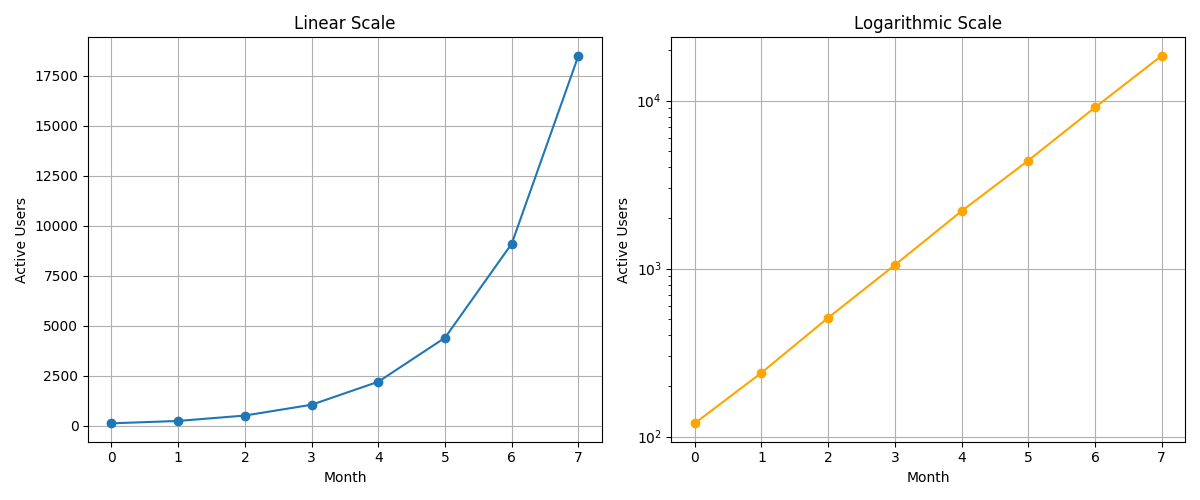
\includegraphics[width=0.97\linewidth]{report_assets/seed_022.png}
\caption{The supplied final artifact for run 022. The separate linear and
logarithmic panels are present; the human label is acceptable.}
\label{fig:run-022}
\end{figure}

\paragraph{Run 079: completed rendering with a different, genuine error.}
The task requests a filled 3D tricontour plot, with a radius range extending
to 1.2, the CMRmap colormap, and an adjusted viewing angle.
Both executions of \texttt{python generate\_plot.py} return zero.
The first emits a Matplotlib deprecation warning, rather than a terminating
exception; the revised script runs with no reported output.
The code saves \texttt{figure.png}, the run ends as \texttt{Submitted},
and the supplied 2340-by-1971 PNG can be decoded.

Importantly, producing this image does \emph{not} mean that the task was
fully satisfied. The final plotting call is a
\texttt{contourf} projection with \texttt{zdir='z'} and a fixed
\texttt{offset=np.min(Z)}. The supplied image shows contour bands on a flat
plane at the bottom of the 3D box, rather than the requested filled 3D
tricontour structure (Figure~\ref{fig:run-079}).
The human label is therefore \texttt{wrong\_chart}, not
\texttt{execution\_failure}.

The baseline instead reports execution failure. Its explanation says
that the script executed without errors and that the figure was saved,
then explicitly states that the answer is \texttt{YES} to indicate that
the agent finished successfully. In particular, it says
\emph{the answer is} \texttt{YES} \emph{to indicate that the agent finished
the task successfully}. The explanation's claim that the
requested chart was fully correct should not be adopted as a fact:
the final artifact and human label show otherwise.
For this run, the baseline incurs an execution FP and a chart FN.

\begin{figure}[htbp]
\centering
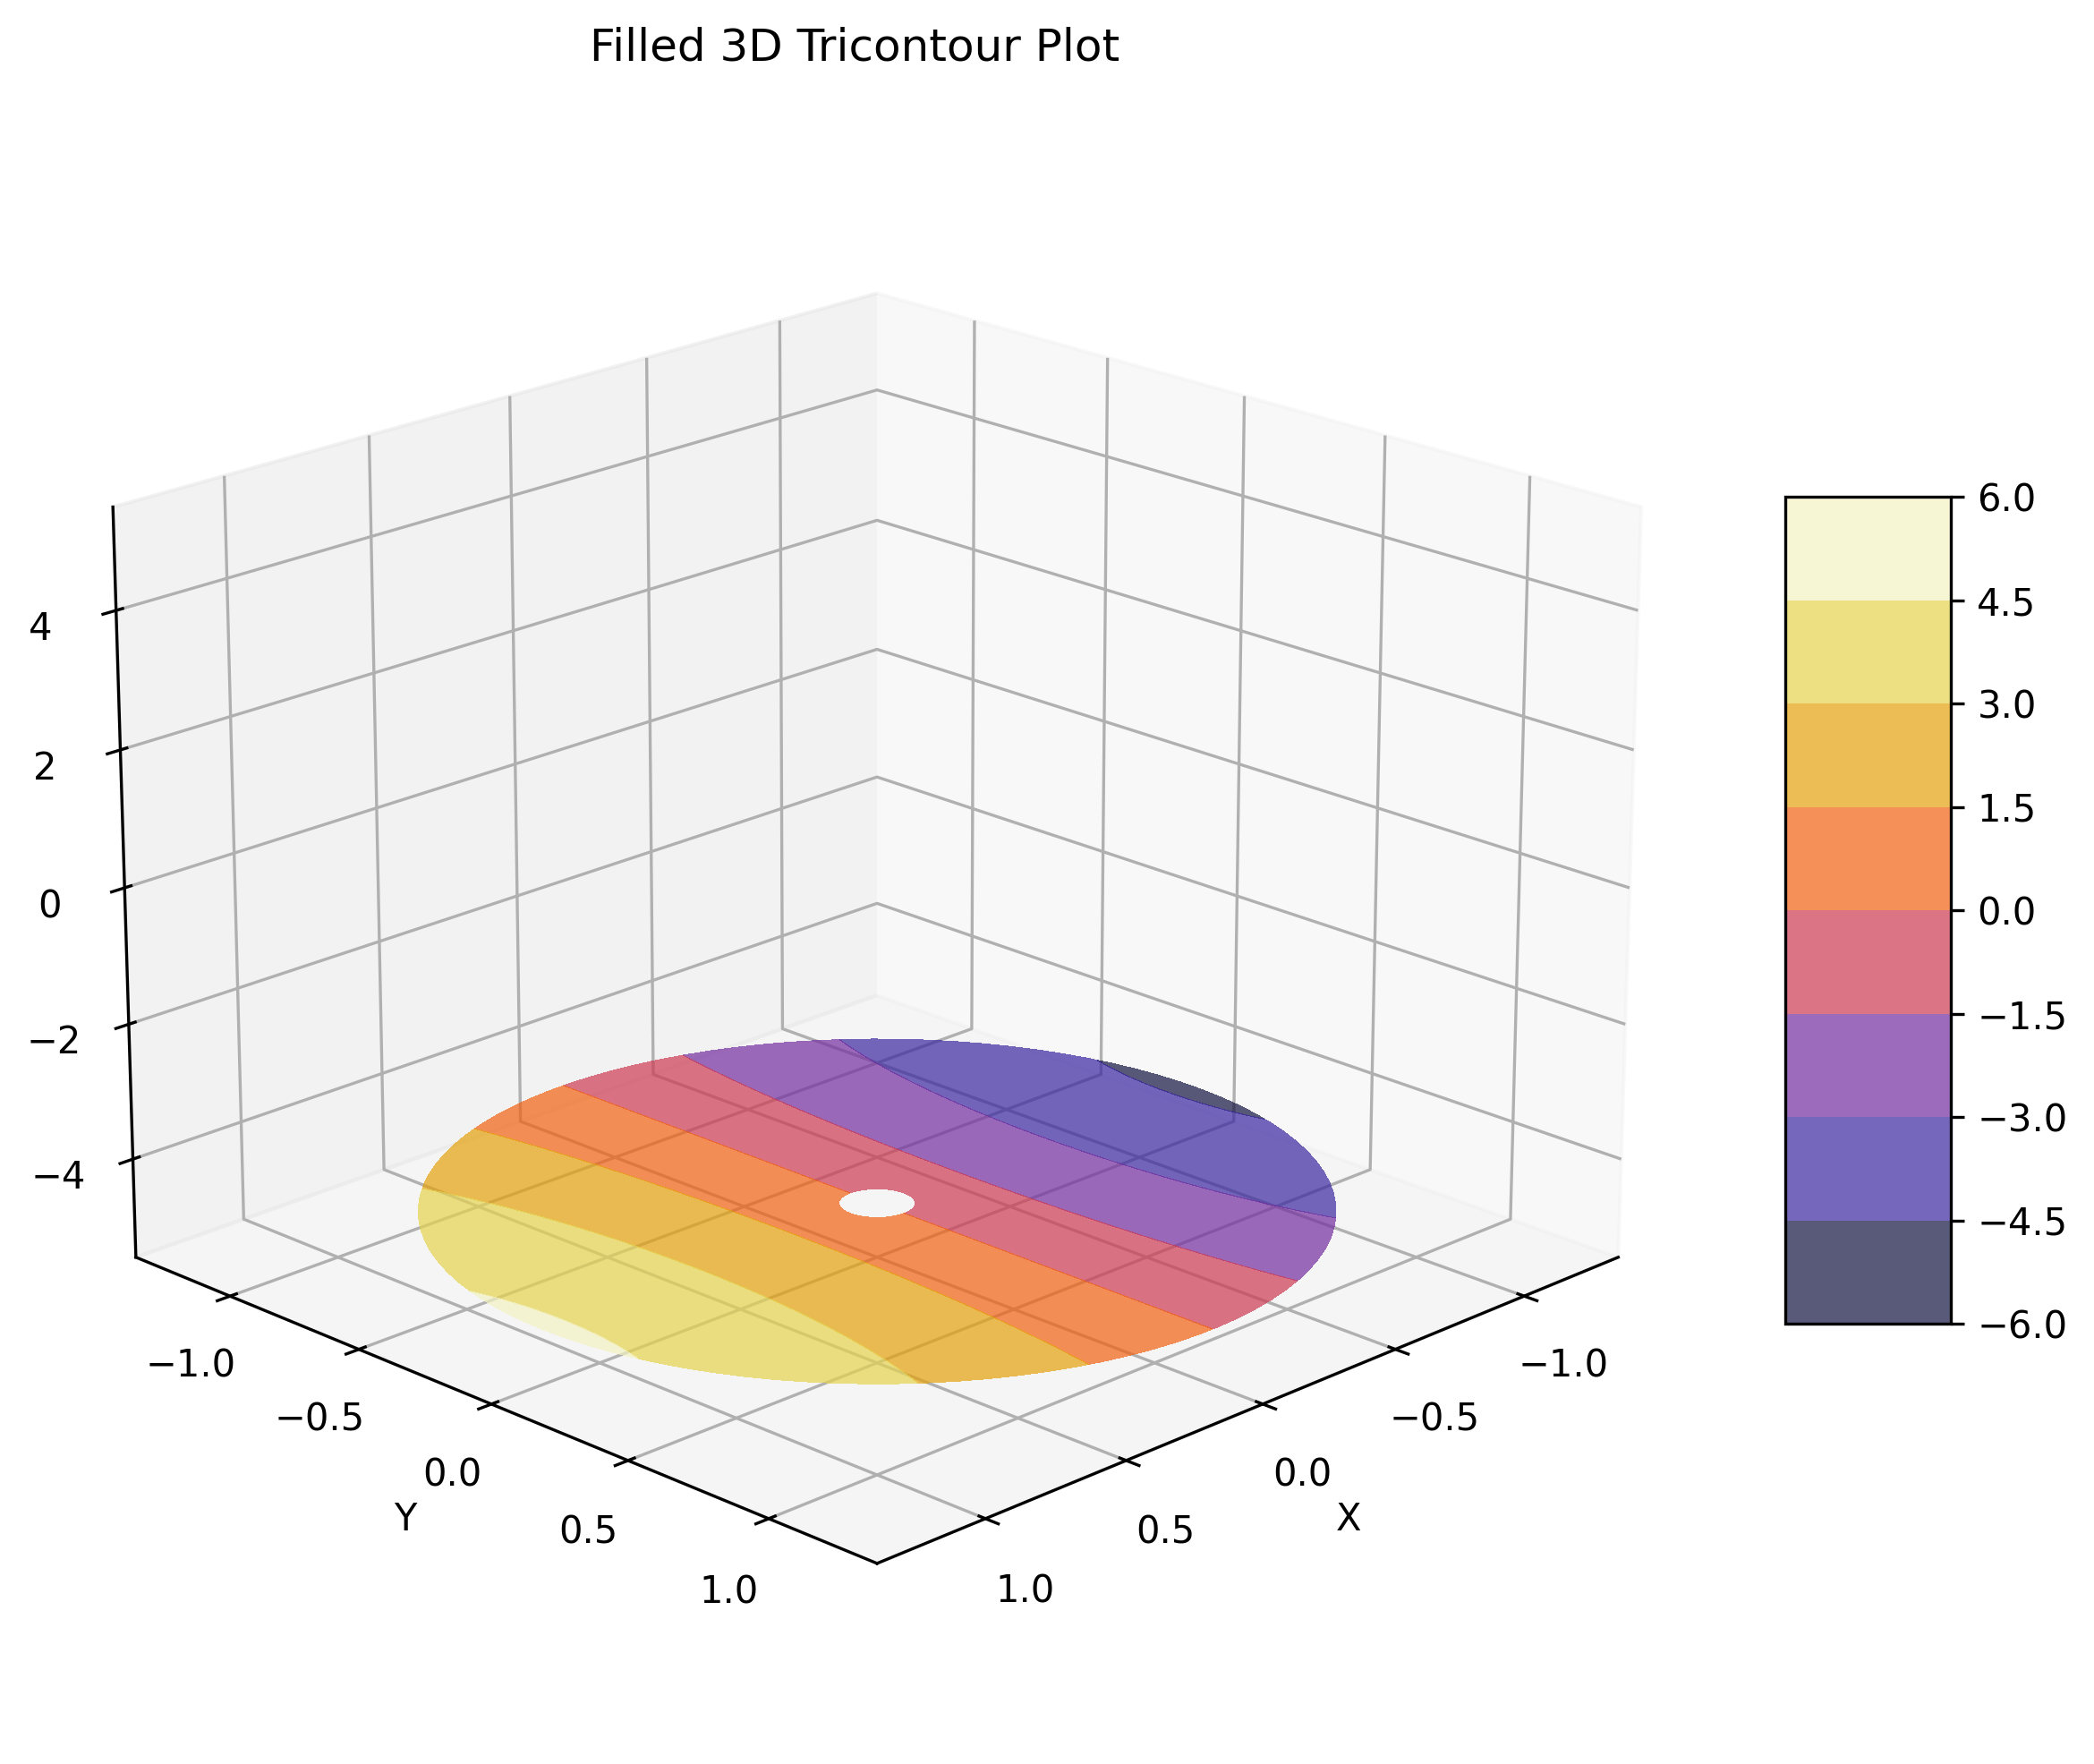
\includegraphics[width=0.68\linewidth]{report_assets/seed_079.png}
\caption{Run 079 delivered a readable PNG, but the contours lie on a fixed
z-plane. This supports the provided \texttt{wrong\_chart} label, not the
baseline's \texttt{execution\_failure} label.}
\label{fig:run-079}
\end{figure}

\paragraph{Implementation-level explanation and downstream consequence.}
In \path{validator/baseline.py}, \texttt{judge\_execution} asks whether
the agent crashed, exhausted its turns, or gave up without producing a
valid figure. The intended answer for successful rendering is \texttt{NO}.
However, \texttt{\_ask} accepts any answer beginning with \texttt{YES} as a
positive for the current error family; it does not check whether the
explanation supports the label. The saved output has already removed the
leading answer token, so I do not claim to have a complete raw-response
log. Run 079's retained explanation nevertheless explicitly documents
the competing interpretation of \texttt{YES} as a success signal.
The relevant source locations are \path{validator/baseline.py}, lines
158--168, for answer parsing and the execution question, and lines
194--198 for the early-return gate.

Finally, \texttt{validate} returns immediately after an execution error.
Thus the incorrect execution decision on 079 suppresses its later chart
check. Correcting the gate would restore the opportunity to evaluate the
chart; it would not by itself guarantee that the chart error is detected.
The evidence supports a mismatch between question polarity, response
meaning, and parsing, rather than a claim that the code reverses every
YES/NO answer or that this mechanism explains every baseline error.

\subsection{Validator Error Type 2}
\label{sec:error-two}

\paragraph{Recurring pattern: explicit axis-label omissions accepted.}
Runs \textbf{021} and \textbf{202} omit axis titles explicitly required
by their tasks, yet the baseline returns \texttt{errors: []} for both.
Their human labels contain \texttt{wrong\_chart}. Neither run is predicted
as an execution failure, so this pattern is distinct from the premature
execution gate in Section~\ref{sec:error-one}.
The common error is a false negative on a concrete design requirement,
not a subjective preference about appearance.

\paragraph{Run 021: tick labels mistaken for a labeled axis in the agent's
self-check.}
The task specifies a vertical box plot for the backend services
\texttt{auth}, \texttt{catalog}, \texttt{search}, and \texttt{checkout},
with the service names as x-tick labels, and separately requires the
chart to \emph{label both axes}. The final image has the y-axis title
\texttt{Latency (ms)} and the four service-name tick labels, but no
x-axis title (Figure~\ref{fig:run-021}).
The last successfully executed version of \texttt{plot\_latency.py}
sets the y-label and title and rotates the ticks, but does not add an
x-label. Its final execution returns zero, and the stored PNG is valid.
Intermediate code errors were repaired; they are not evidence of a
final execution failure.

The human label identifies the missing x-label as \texttt{wrong\_chart},
whereas the baseline returns an empty error list.
The agent's final self-check lists the service names as \emph{X axis labels},
illustrating the distinction that must be verified: tick labels identify
individual categories, whereas an axis title identifies the axis.
The task did not prescribe a particular x-axis-title string, so the
violation is absence of a title, not failure to use an invented exact phrase.

\begin{figure}[htbp]
\centering
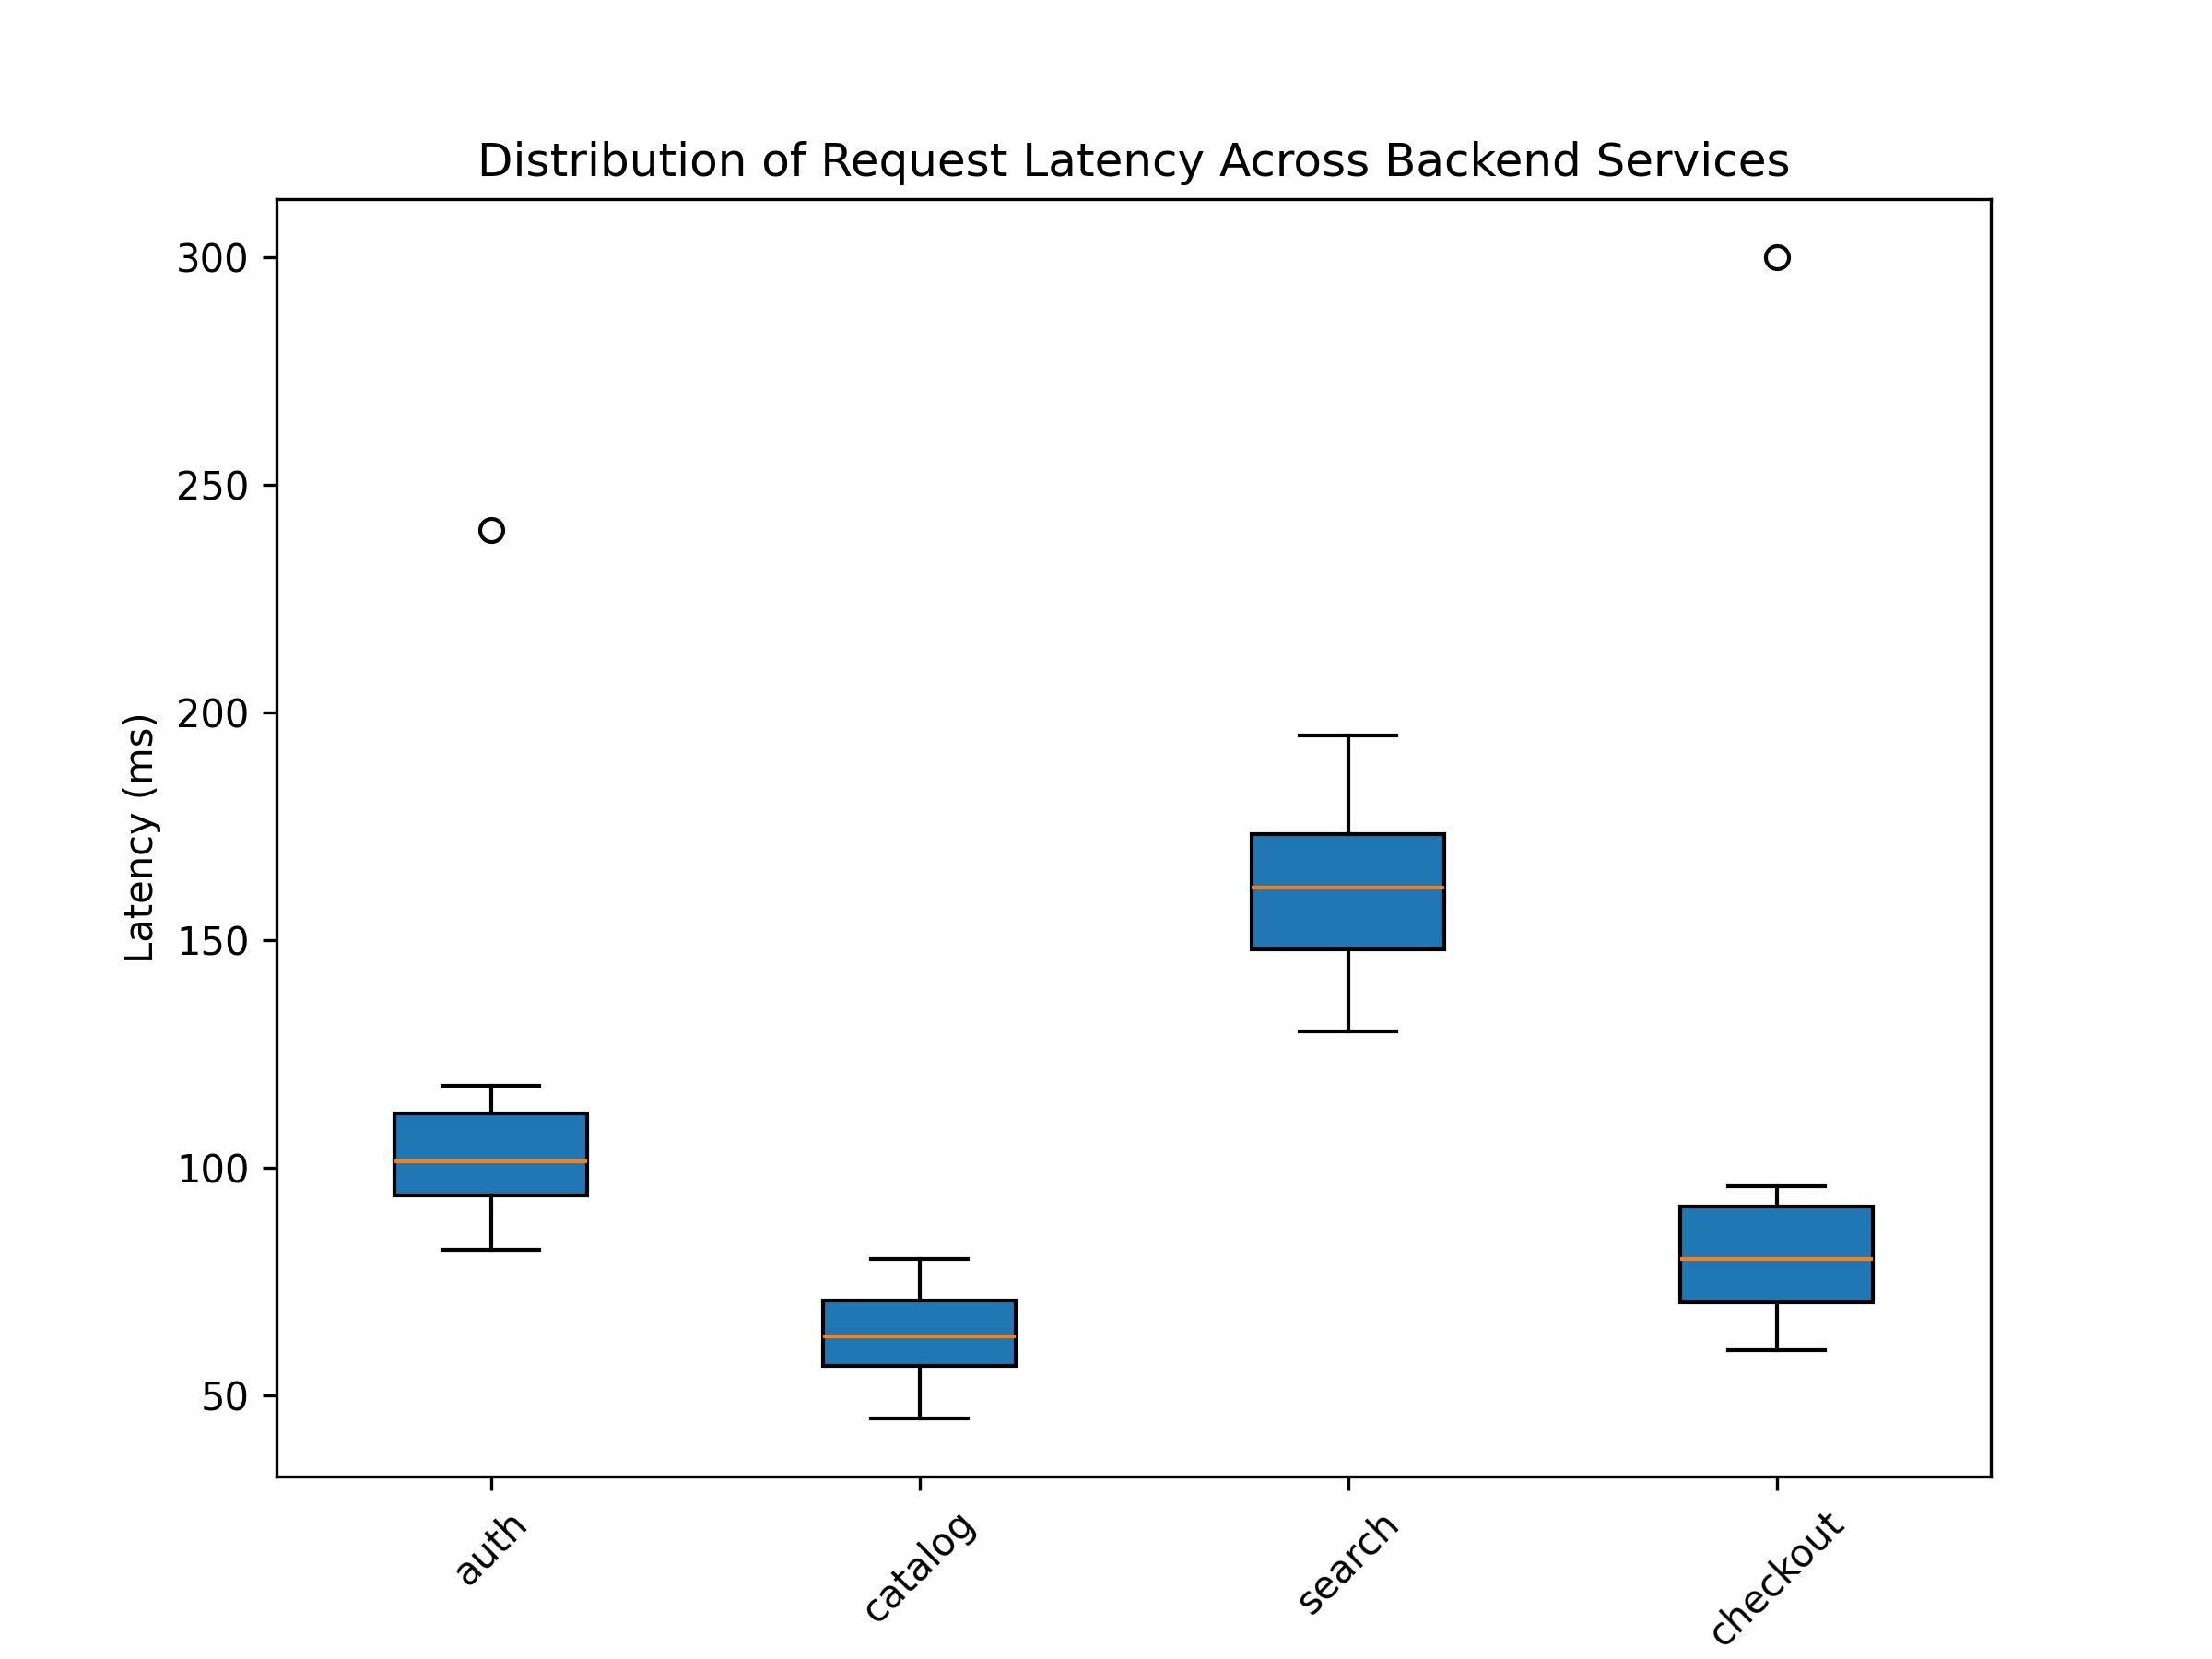
\includegraphics[width=0.70\linewidth]{report_assets/seed_021.png}
\caption{Run 021 has service-name tick labels and a y-axis title, but no
x-axis title despite the explicit requirement to label both axes.}
\label{fig:run-021}
\end{figure}

\paragraph{Run 202: required labels lost in the final script.}
The task asks for standard and notched box plots in a 1-by-2 layout,
with the x-axis label \texttt{Four separate samples}, the y-axis label
\texttt{Measured values}, and horizontal gridlines in both panels.
The final image retains the x-labels, but neither panel displays the
required y-label; neither displays the requested gridlines
(Figure~\ref{fig:run-202}).
The human label records these two chart-design omissions, but the
baseline again returns an empty error list.

The trajectory is particularly informative. An earlier
\texttt{generate\_boxplots.py} includes the y-labels and gridlines.
Later, the agent writes a new \texttt{plot.py}; that final script retains
\texttt{set\_xlabel} but omits \texttt{set\_ylabel} and the grid calls.
It then successfully runs \texttt{python plot.py}, saves to
\texttt{figure.png}, and submits. The last script and the supplied final
image therefore corroborate the omissions.
An earlier successful script cannot establish compliance after a later
script has regenerated the output.

\begin{figure}[htbp]
\centering
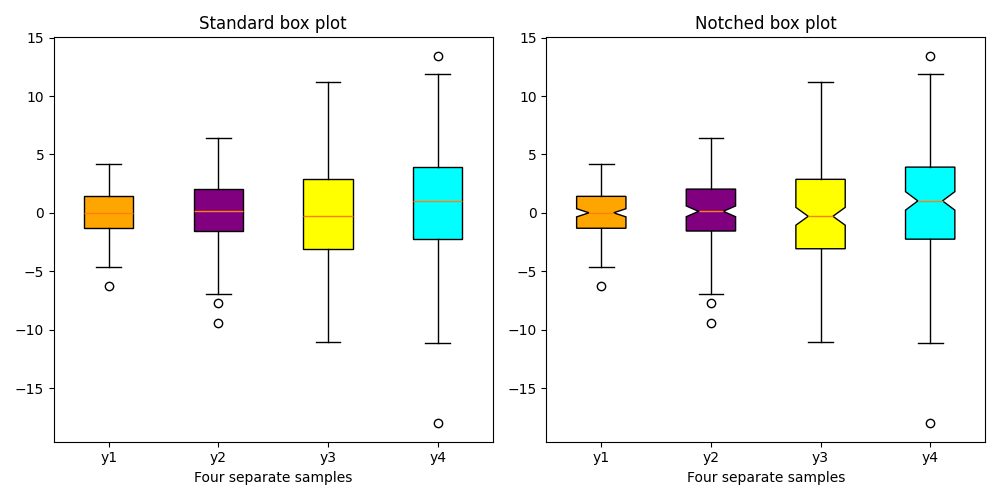
\includegraphics[width=0.97\linewidth]{report_assets/seed_202.png}
\caption{Run 202 retains the x-axis labels, but the specified
\texttt{Measured values} y-axis labels and horizontal grids are absent
from both final panels.}
\label{fig:run-202}
\end{figure}

\paragraph{Why a different check is needed.}
The baseline asks a single broad question about whether the figure follows
the requested chart design. It does not require an explicit audit of each
requirement or identification of the final output-producing script.
The two examples demonstrate that this procedure failed to detect
clear axis-label omissions even when a figure was available.

Possible contributing factors are confusing tick labels with axis titles,
trusting the agent's self-description, or treating earlier correct code as
evidence about the final figure. These are hypotheses motivated by the
observed trajectories, not claims about the judge's hidden reasoning.
In particular, the empty predictions do not preserve the negative
responses, so it would be unsupported to quote an invented model
explanation for either run.

\subsection{Proposed Validator Changes}
\label{sec:proposals}

The following changes were \emph{proposed} after the baseline analysis.
This section records their motivation before implementation; the incremental
implementation and validation status is recorded separately in Part 2.
No improved-validator scores are claimed in Part 1.

\paragraph{Change 1: artifact-grounded execution decisions with explicit
failure polarity.}
Replace the bare YES/NO execution interface with an explicit internal
decision field, such as \texttt{execution\_failure: true/false}, plus
specific supporting evidence. Define \texttt{true} only as failure to
deliver a valid final figure, and \texttt{false} as permission to continue
the remaining three checks, not as an assertion that the whole task is
correct. Strictly validate the response schema and Boolean type rather
than relying on a leading word or converting arbitrary strings to truth
values.

Ground the decision in the actual final artifact and trajectory:
check whether the required image exists and can be decoded, and examine
the final relevant tool results and output path. These filesystem and
decoding checks are deterministic evidence; the interpretation of the
trajectory and rendered content can remain model-based. A decodable PNG
alone is not proof of correct data, correct design, or readability.
Likewise, \texttt{Submitted} and an agent-written success claim are not
sufficient proof, and a repaired intermediate exception does not establish
final failure.

A malformed or contradictory judge answer should trigger bounded
rechecking or retry. If a reliable judgment cannot be obtained, raise a
validator-side error so the existing runner can retry, rather than
silently treating the run as acceptable or labeling the visualization
agent as an execution failure. Do not invert labels merely because an
explanation contains a word such as \emph{success}.
When execution really fails, retain the terminal-family convention;
otherwise, continue all three nonterminal checks.
This targets the documented polarity mismatch in 022 and 079 while
preserving the distinction between delivery and task compliance.

\paragraph{Change 2: requirement-by-requirement audit of the final chart.}
Extract the task's explicit chart-design requirements into a checklist,
including their scope (which panel, axis, or whole figure they apply to).
For each requirement, compare the final rendered figure with the last
relevant output-producing code and tool results, recording a status such
as pass, fail, or uncertain and concrete evidence.
Explicitly distinguish axis titles from tick labels and verify exact
text only when the task specifies exact text. Do not impose an additional
x-label phrase on 021; do check \texttt{Measured values} on 202.

The final image is the evidence of what was actually rendered.
Trace the full tool-call sequence to identify later overwrites rather
than searching the entire trajectory for any earlier occurrence of a
correct plotting call. Code inspection is corroboration, not a universal
static rule: labels may be produced by helper functions, shared figure
labels, or other valid plotting APIs. Whether a shared label is sufficient
depends on the task, not on an unconditional requirement to repeat every
label on every panel.
The agent's statement that requirements are satisfied is not a substitute
for this audit.

Uncertain items should receive targeted additional inspection with the
same fixed judge model, rather than automatically passing. Confirmed
design violations should be consolidated into one
\texttt{wrong\_chart} error with specific evidence; for 202, that evidence
can mention both the missing y-label and gridlines. This keeps category
boundaries intact: missing required labels are chart errors, not
execution failure, and missing text is not automatically a readability
error. Formatting or request failures must not be hidden as ordinary
uncertainty and then converted into an empty error list.
This proposal specifically targets the axis-label false negatives in
021 and 202, while the checklist mechanism generalizes to other explicitly
requested design elements.

\paragraph{Constraints and validation plan.}
Both changes are restricted to the student validator while
preserving \texttt{validate(run)} and the required list-of-errors output
schema. The internal decision/checklist protocol does not replace the
external \texttt{family}/\texttt{evidence} contract.
All model-based steps will use the fixed Qwen3-VL judge; no other model
will be called. The validator will operate on the current run's evidence,
without loading \path{seed_labels.json}, using run-ID lookup tables, or
consulting other candidate runs to choose a prediction.
The original baseline and its prediction file will be preserved as the
comparison point.

Part 2 will test whether the changes reduce the targeted errors on the
four case-study runs and on the complete seed set. It must also check
for regressions: check and report whether execution false negatives increase
because the new check is too permissive, or whether the checklist invents
requirements or rejects permitted shared labels.
All four family MCCs and macro-MCC will be compared with
Table~\ref{tab:baseline}, alongside at least one remaining FP and FN.
Structured output can still contain an incorrect semantic judgment,
and a stricter evidence threshold can increase omissions; therefore,
neither proposal is presented as a guaranteed improvement or as a
demonstrated solution to the private grading set.

\clearpage
\section{Part 2: Improve Your Validator}

\subsection{Implemented Changes}

\paragraph{Completed Part 2 scope.}
Both proposed changes have been implemented in \path{validator/solution.py}.
The original \path{validator/baseline.py} and
\path{output/baseline_predictions.json} remain unchanged.
The execution gate and chart-design check are replaced; the data and
readability checks retain the baseline procedures. The implementation is
runnable and has been evaluated on all 110 released seed runs. The incremental
tests below document development checks; the full results in
Section~\ref{sec:part2-performance} are the primary performance comparison.

\paragraph{Change 1: deterministic artifact checks.}
The execution gate first reads the actual delivered image. No recorded image
path, a missing file, a directory in place of the file, an invalid PNG format,
or a corrupt PNG yields a terminal \texttt{execution\_failure} with specific
artifact evidence. A present image must pass both Pillow's structural
\texttt{verify()} check and a fresh open with \texttt{load()} to decode pixels.
The implementation does not search for an alternative output path or execute
the agent's plotting code to repair the delivered artifact.
Permission and file-reading environment errors propagate to the runner rather
than becoming an agent-failure label. Thus a successful shell command or an
agent-written completion claim cannot compensate for a missing required output.

\paragraph{Change 1: model-based delivery judgment and strict parsing.}
For a decodable PNG, the same fixed Qwen3-VL model receives the task, input-file
contents, full serialized trajectory including tool calls and tool results,
and the image. The instructions separate final delivery from data correctness,
chart design, and readability, and explicitly disregard repaired intermediate
exceptions as evidence of final failure. A blank-looking image alone is not
enough to diagnose execution failure: invisible plotted elements may instead
be a readability problem. For a positive judgment about a decodable artifact,
the prompt requires image and trajectory evidence that it is only a placeholder
or an unrelated non-figure artifact; this requirement is not a programmatic
proof of the model's evidence.

The internal response has exactly three fields:
\texttt{execution\_failure}, \texttt{artifact\_status}, and \texttt{evidence}.
Only a real JSON Boolean is accepted. The status must be
\texttt{rendered\_figure} when failure is false, or
\texttt{no\_figure\_content} when failure is true.
Unknown or missing fields, duplicate keys, blank evidence, malformed JSON,
and responses truncated at the output limit are rejected.
A single enclosing JSON code fence is tolerated, but explanatory text outside
the JSON is not. The public return type remains \texttt{list[Error]}, with the
unchanged \texttt{family}/\texttt{evidence} schema.

There are at most two decision attempts for a decoded artifact, excluding
transport retries and context-overflow handling. A valid false decision
permits the remaining three family checks. A provisional true decision is
rechecked against the category boundary and must be confirmed before returning
an execution error. If the attempt budget expires without a reliable decision,
the function raises a validator-side error for the runner, rather than
guessing an agent label or returning an empty error list.
The parser checks consistency between the structured fields; it cannot prove
that all natural-language evidence is semantically consistent or that the
model's judgment is correct. The second judgment is a targeted recheck, not an
independent ground-truth oracle.

\paragraph{Context handling and scope.}
The model client retains temperature zero, and execution judgments allow
512 output tokens. Full evidence is attempted first. Only a recognized context
overflow triggers compaction using the server's reported context limit and
tokenizer. The compacted text budget reserves half the context for the image
and formatting and explicitly reserves the execution response budget.
Input text may retain only its beginning and end. Trajectory compaction retains
a chronological suffix of complete messages, normally considering up to the
last 12, and preserves the last tool call/result group whose IDs can be linked.
It does not retain a known tool result without its caller. If even the required
final group cannot fit, the context error is surfaced.
Earlier events, including some output-producing code, can still be omitted;
this is not a guarantee that all relevant history survives.
Omissions are disclosed to the judge and must not be interpreted as agent errors.
If necessary, the existing baseline helper downscales the request image
in memory; the supplied on-disk figure is never replaced.

All decisions use only the current run. The submitted validator does not load
human labels or branch on public run IDs. The selected IDs below belong only
to the separate test harness. The Step 2.1 experiment below predates the
separate design-audit implementation and concerns only the execution gate;
its recorded \texttt{implementation\_sha256} identifies that earlier version,
not the current two-change source.

\paragraph{Incremental local verification.}
The offline regression suite in \path{tests/test_solution_execution.py}
contains 33 passing tests, with model and tokenizer responses mocked.
It covers strict parsing, bounded rechecking, PNG validation, repaired
exceptions, propagation of validator-side failures, terminal early return,
and preservation of the nonterminal output schema. Context tests include
oversized early history and a final tool group followed by completion messages;
if only the completion message fits, the check must raise rather than silently
drop the final known tool group.
These are tests of program behavior, not evidence that the real judge always
classifies synthetic blank or invisible charts correctly.

The read-only artifact audit in \path{tests/check_execution_smoke.py} inspected
all 110 released runs: 12 have no delivered \texttt{figure.png}, and 98 PNGs
pass structural verification and full decoding.
Comparison with the provided labels confirms that those 12 missing outputs
are the 12 human-labeled execution failures. This comparison is performed for
offline evaluation only; labels are not input to the validator.
The audit does not measure the model-based gate's predictions on the 98 images
and must not be interpreted as a full-validator MCC result.

The local checks can be reproduced without model requests:
\begin{verbatim}
uv run python -m unittest discover -s tests \
  -p test_solution_execution.py
uv run python tests/check_execution_smoke.py
\end{verbatim}

\paragraph{Limited real-model smoke test.}
The execution gate alone was then tested on six selected released runs.
The saved diagnostic record is
\path{tests/diagnostics/step2_1_execution_checks.json}; it explicitly identifies its scope
as execution-only and stores the actual judge responses and token usage.
This is not the full prediction file required for Part 2.
The test can be reproduced with the existing validator endpoint:
\begin{verbatim}
uv run python tests/check_execution_smoke.py \
  --live --run-ids 022 079 021 202 089 105
\end{verbatim}
The five runs with PNGs each obtained a valid false execution decision on the
first model call. Run 089 was rejected locally for its missing required output,
without a model call. The five completed judge calls used 43,734 total tokens
as reported by the service, including 751 completion tokens.
No context-overflow or response-repair path was needed in this selected test.

\begin{table}[htbp]
\centering
\small
\begin{tabular}{lcccc}
\toprule
Run & Human & Baseline & Step 2.1 & Model calls \\
\midrule
022 & No  & Yes & No  & 1 \\
079 & No  & Yes & No  & 1 \\
021 & No  & No  & No  & 1 \\
202 & No  & No  & No  & 1 \\
089 & Yes & No  & Yes & 0 \\
105 & No  & Yes & No  & 1 \\
\bottomrule
\end{tabular}
\caption{Execution-failure decisions only: Yes means this family is present,
not that the task is successful. All six selected execution decisions agree
with the human labels. These are targeted examples, not an unbiased performance
estimate or a complete four-family evaluation.}
\label{tab:execution-smoke}
\end{table}

The targeted execution false positives on 022 and 079 are absent in this
smoke test. Run 105 adds another repaired-exception example: the baseline
reports execution failure even though the final plot was delivered; the new
gate permits further checks. Conversely, run 089 illustrates a corrected
execution false negative. Its trajectory records successful plotting code
that saves \texttt{plot.png}, but the required \texttt{figure.png} was not
delivered. The new deterministic check diagnoses the actual missing output
instead of adopting the completion claim.

The smoke test also exposes a remaining limitation rather than proving all
judge reasoning reliable. For 079, the model's internal false-decision
explanation calls the chart a filled 3D tricontour, despite the flat contour
projection discussed in Part 1. For 202, it incorrectly claims that the final
chart has the required y-axis label and horizontal gridlines.
Those details conflict with the supplied image and final plotting code.
The delivery decisions are nevertheless correct: both runs have figures.
Their internal explanations must not be reused as evidence that the design
requirements pass. This motivates keeping the separate design audit in
Change 2, rather than allowing a negative execution decision to certify
the entire task. Passing the execution gate on 021 and 202 does not resolve
their chart-design false negatives; Change 2 is tested separately below.

\paragraph{Change 2: task-only, scoped requirement extraction.}
The fixed judge first receives only the original task instructions and their
numbered nonempty lines, not the candidate's image, trajectory, or completion
claims. The policy instructs it to extract individually checkable, explicit
requirements for chart type/projection, layout, axes,
legend/colorbar/annotations, and style. Each item records a unique ID, kind,
requirement, affected panel/axis scope, and source-line ID. The implementation
restores that line's verbatim text as the item's source quotation.
The parser rejects unknown source IDs, extra/missing fields, invalid kinds,
duplicate requirement IDs, and empty/non-string fields. A response using a
source quotation instead of an ID is also accepted only when it passes the
original strict quotation checks; it cannot bypass grounding.
This prevents successful ID-based responses from rewriting quotations, but
does not prove that their interpretations are supported by those lines or
that extraction is complete. An omitted requirement, wrongly inferred scope,
or an unsplit compound item remains a possible source of false negatives:
atomic splitting is requested in the policy, not proved by the parser.

The extraction policy prohibits inventing unrequested labels, grids, legends,
exact wording, or dimensions. It separates numerical correctness from design
requirements. An axis label is not interchangeable with category tick names.
Panel scope matters: a requirement for both panels cannot be satisfied by
checking only one. An empty checklist is allowed for a task with no explicit
design requirements; this too relies on the model's extraction judgment.

\paragraph{Change 2: unprimed observation and final-artifact audit.}
Before an audit, a separate call receives only the final image, without task
text, expected labels, input contents, or agent claims. It describes visible
panel positions, titles, separate axis labels versus tick labels, grids,
annotations, and geometry. This is a fallible observation by the same fixed
model, not a reference figure or an independent oracle. Its purpose is to
reduce substitution of expected elements for observed ones.

The audit then receives that observation, the checklist, original task, input contents, full
serialized trajectory, and decoded final PNG. The policy makes visible final
image evidence primary and uses the latest successfully executed
output-producing code to corroborate metadata and ambiguities.
Correct earlier code and agent success claims do not certify the final
artifact. This directly addresses the overwritten-script pattern in 202.
Equivalent implementations, including pyplot functions, helpers, and
shared/global labels when allowed by the task, are accepted; the validator
does not decide label absence by searching for one API name.

Each checklist ID must appear exactly once in the audit with one of
\texttt{pass}, \texttt{fail}, or \texttt{uncertain}, plus nonempty evidence.
Missing, duplicate, or unknown IDs are rejected, not silently counted as
passing. Only uncertain items receive one targeted recheck round.
Confirmed failures are consolidated into one \texttt{wrong\_chart} error,
whose evidence includes each violated requirement, scope, task quote, and
final-state observation. If no failure is established but an item remains
uncertain, the check raises a validator-side error instead of claiming success.
When a confirmed failure already establishes this binary family, it remains
reportable even if another requirement is unresolved; the unresolved item is
not presented as a demonstrated violation.

Both extraction and each audit allow at most two response-format attempts.
Truncation, malformed JSON, invalid fields, and incomplete coverage trigger
schema repair; exhausting the budget propagates an error.
Transport and unavailable-context failures do not become agent labels.
Extraction allows 3,072 output tokens, image-only observation 1,024,
and audit 4,096. Observation also rejects empty/non-textual or truncated
responses with a bounded retry; non-context service errors propagate.
The audit's context fallback budgets the full task, checklist, stage policy,
and actual response allowance, rather than reusing the execution check's
512-token response reservation. The task and checklist are never excerpted.
Trajectory/input omissions and possible in-memory image downscaling retain
the limitations described above.

To reduce persistent formatting failures observed during development,
extraction and audit also request JSON-schema-constrained decoding through
the existing fixed-model endpoint, following the
\href{https://docs.vllm.ai/en/v0.15.0/features/structured_outputs/}
{vLLM structured-output interface}.
The extraction schema limits source IDs and kinds to their current-task
allowed values. The audit schema allows only ID, status, and evidence,
restricts IDs to the supplied checklist, and requires its number of entries.
Local parsers still verify nonempty fields, unique IDs, and exact coverage.
Format constraints do not prove correct interpretation, complete extraction,
truthful visual evidence, or correct error-family attribution.
No server deployment, model, runner, or external prediction schema was changed.

Data correctness still uses the baseline's independent data-only question.
The old combined data-and-chart helper is not called, preventing duplicate
or contradictory chart judgments. Data and design errors can coexist.
Readability remains a separate baseline check.
For a delivered chart without repairs or uncertainty, this version normally
makes six calls: execution, data, requirement extraction, image-only
observation, design audit, and readability.
The additional calls are a cost of explicit coverage, not evidence
that the underlying fixed model is infallible.

\paragraph{Change 2: offline regression tests.}
The combined suite now has 91 passing tests: the 33 execution tests above
and 58 design tests in \path{tests/test_solution_design.py}.
Design tests cover grounded quotations, strict schemas and exact checklist
coverage, bounded format repair, rejection of truncated answers, independent
data/design labels, uncertain-item rechecking, and unresolved-error propagation.
Mocked interface tests verify that extraction receives only task instructions,
whereas audit receives exact final-image bytes, raw tool calls/results, and
input contents. Context tests verify the design-specific policy and response
budget, checklist preservation, non-context error propagation, and image
downscaling without changing the on-disk figure.
Additional tests verify task-line ID restoration, image-only observation
isolation and bounded retries, JSON-schema request parameters, targeted
subset schemas, and unchanged format constraints during context fallback.
A mocked shared-label case checks control-flow compatibility with an
allowed global label; it is not a real-model generalization result.

\begin{verbatim}
uv run python -m unittest discover -s tests \
  -p 'test_solution_*.py'
\end{verbatim}

\paragraph{Targeted development checks and limitations.}
The design-only harness \path{tests/check_design_smoke.py} was run on seven
selected seed cases, not on the entire seed set. Its scope deliberately
excludes execution, data, and readability classification.
Early development checks exposed missed design requirements, rewritten source
quotations, and audits that repeatedly copied extra checklist fields.
These motivated source-line IDs and schema-constrained decoding.
Such validator-side operational failures were not counted as negative labels.
The superseded debug records are not used for the full-set results below.

The final selected test is saved in
\path{tests/diagnostics/step2_2_design_checks.json}.
Its recorded source hash matches the tested implementation.
It completed all seven cases using 21 model calls, with 94,815 service-reported
total tokens, including 9,183 completion tokens.
Each case used one extraction, one image-only observation, and one audit;
no format repair, uncertainty recheck, or context fallback was needed in this
final selected test. The command is:
\begin{verbatim}
uv run python tests/check_design_smoke.py \
  --live --run-ids 021 202 022 105 079 097 196
\end{verbatim}

\begin{table}[htbp]
\centering
\small
\begin{tabular}{lccc}
\toprule
Run & Human wrong-chart & Baseline wrong-chart & Step 2.2 wrong-chart \\
\midrule
021 & Yes & No & Yes \\
202 & Yes & No & Yes \\
022 & No  & No & No  \\
105 & No  & No & No  \\
079 & Yes & No & No  \\
097 & No  & No & No  \\
196 & No  & No & No  \\
\bottomrule
\end{tabular}
\caption{Design-family membership only on selected cases.
Baseline 079 and 105 instead return execution errors; No in their
design column does not imply overall task success.
These targeted observations are not a full-validator MCC estimate.}
\label{tab:design-smoke}
\end{table}

The final selected smoke-test labels recover the targeted design positives on
021 and 202, and
all four selected design-negative controls remain negative.
The controls exercise acceptable linear/log labeling (022), no unrequested
figure-size constraint (105), pyplot-based labels and a plotted maximum
marker (097), and a task that requires a y-axis label but not an x-axis label
or a grid (196). These examples do not establish hidden-set generalization.

Critically, correct binary labels do not make every explanation correct.
For 021 the new evidence correctly identifies the absent separate x-axis
label, but it also wrongly insists that the valid label \texttt{Latency (ms)}
must literally read \texttt{latency in milliseconds}. The task specifies the
quantity and unit, not that exact string.
For 202 the final audit flags the grid requirement, but hallucinates vertical
gridlines: the supplied image has no gridlines. It also incorrectly passes
the missing \texttt{Measured values} labels.
Image-only observations themselves sometimes hallucinate elements, and the
later audit can repeat those claims or prefer earlier correct code.
These failures remain despite valid schemas and grounded source IDs.

Run 079 remains a design false negative: the model accepts a flat contour
projection on 3D axes as the requested filled 3D tricontour plot.
The observation even describes both varying height and a single flat plane,
illustrating unresolved semantic inconsistency. Consequently, this step
supports limited improvement in family detection, not a claim that final
code provenance, task interpretation, or image grounding is solved.
The complete experiment below provides all four family scores and analyzes
actual full-run false positives and false negatives. In particular, these
selected smoke-test outcomes must not substitute for the full-run results.

\subsection{Seed-Set Performance vs.\ Baseline}
\label{sec:part2-performance}

\paragraph{Experiment and coverage.}
The two-change validator was run on the entire released seed set, using the
same fixed model and the unchanged public runner and prediction schema.
The saved \path{output/pre_iteration_seed_predictions.json} contains exactly
110 predictions with 110 unique run IDs, matching the human-label IDs with no
missing or additional runs. The official scorer validates the prediction
schema. Each returned error has one of the four prescribed families and
nonempty evidence. The reproduction commands are:
\begin{verbatim}
uv run python -m validator.runner \
  --artifacts artifacts \
  --out output/pre_iteration_seed_predictions.json

uv run python -m workflow score \
  --labels seed_labels.json \
  --predictions output/pre_iteration_seed_predictions.json
\end{verbatim}
The baseline comparison uses the separately preserved
\path{output/baseline_predictions.json}; it is not regenerated with the new
implementation. Labels are used only by offline scoring and analysis, never
as validator inputs.

The unchanged Part 2 source at this checkpoint has SHA-256:
\begin{verbatim}
7b968ed3ccccbcc9b2fa6fb0f69f314453913ace8b0c41e1a4649495a0627551
\end{verbatim}
This also matches the source hash in the final design-only diagnostic record.
The full prediction JSON itself does not contain per-stage judge responses,
token counts, timings, or a source-hash field; the hash above identifies the
preserved implementation, not additional metadata embedded in that JSON.
The Part 2 prediction file is retained separately from subsequent Part 4
predictions.

\begin{table}[htbp]
\centering
\small
\begin{tabular}{lrr}
\toprule
Metric & Baseline & Part 2 \\
\midrule
\texttt{execution\_failure} & $-0.0022$ & $1.0000$ \\
\texttt{wrong\_data}        & $0.0000$  & $-0.1445$ \\
\texttt{wrong\_chart}       & $0.1096$  & $0.3512$ \\
\texttt{hard\_to\_read}     & $0.0000$  & $-0.2424$ \\
\midrule
Macro-MCC                  & $0.0268$  & $0.2411$ \\
\bottomrule
\end{tabular}
\caption{Full-seed comparison using the official scorer; MCC values are
rounded to four decimal places. Higher is better, and negative values indicate
negative correlation, not merely a low accuracy percentage.}
\label{tab:part2-mcc}
\end{table}

\begin{table}[htbp]
\centering
\small
\begin{tabular}{lrrrrr}
\toprule
Family & Evaluated runs & TP & TN & FP & FN \\
\midrule
\texttt{execution\_failure} & 110 & 12 & 98 & 0 & 0 \\
\texttt{wrong\_data}        & 98  & 2  & 58 & 15 & 23 \\
\texttt{wrong\_chart}       & 98  & 41 & 22 & 5 & 30 \\
\texttt{hard\_to\_read}     & 98  & 0  & 51 & 8 & 39 \\
\bottomrule
\end{tabular}
\caption{Part 2 confusion counts. The 12 human-labeled execution failures are
excluded from the other families, as required by the scoring rule; a predicted
execution failure would not exempt a nonterminal gold run from evaluation.}
\label{tab:part2-confusion}
\end{table}

\paragraph{Interpretation and regressions.}
Macro-MCC increases from approximately 0.0268 to 0.2411. The execution gate
eliminates all 33 baseline execution false positives and all eight execution
false negatives on this seed set. The design family detects 41 of 71 positive
runs, rather than the baseline's three, but also introduces five false
positives. Thus the overall increase does not mean that every family improves:
data detects only two of 25 positives with 15 false positives, while readability
detects none of 39 positives with eight false positives. Both resulting MCCs
are negative.

The unchanged data/readability procedures now run on candidates that the old
execution gate rejected early. All 15 new data false positives and all eight
new readability false positives lie among those 33 baseline execution false
positives. This is an observed relationship between saved predictions, not
proof that each model judgment was otherwise identical across experiments.
It shows why correcting a terminal gate can expose downstream weaknesses.
There is no ablation that separates the contributions of the gate and design
audit; the reported gains belong to the complete two-change pipeline.

\paragraph{Runtime and context limitations.}
For an ordinary delivered chart, the new pipeline normally makes six model
calls rather than the baseline's four. The old baseline also stopped early
on many valid charts, whereas Part 2 checks all three nonterminal families
on those charts. Larger structured design responses, retries, model/container
startup, and context fallback can add runtime. The prediction file does not
record the full run's actual call count, cost, or wall time, so the selected
smoke-test token totals above are not extrapolated as measured full-run totals.

A context-overflow warning was observed during the full evaluation. The
implementation attempts its documented compaction/downscaling fallback;
the completed file has full coverage and valid schema. This establishes
completion, not preservation of every original detail after fallback.
The saved predictions do not identify the final retained context or resolution
for each stage. Consequently, I do not attribute a particular false negative
to that warning. Loss of earlier code, omitted input rows, or lower image
resolution remain general risks of the fallback.

\subsection{Qualitative Analysis of Targeted Error Types}

\paragraph{Error type 1: execution polarity and final delivery.}
The full evaluation confirms the targeted gate improvement, not just the
selected smoke test. Runs 022 and 079 are no longer labeled execution failures:
both have decodable delivered plots, despite the baseline's false-positive
execution judgments. Run 089 now receives only the terminal execution label
because its required output is missing, even though its trajectory contains
successful code that saved a differently named file.
Together with the full confusion counts, these outcomes support mitigation
of the Part 1 execution pattern on the released set. They do not establish
perfect performance on unseen decodable placeholders or corrupted artifacts.

Removing an execution error does not guarantee overall correctness. Run 022
now has a spurious data label, and run 079 still has an undetected design error.
The table summarizes the full predictions for the original four examples:
\begin{table}[htbp]
\centering
\small
\begin{tabular}{lccc}
\toprule
Run & Human families & Baseline families & Part 2 families \\
\midrule
022 & None  & Execution & Data \\
079 & Chart & Execution & None \\
021 & Chart & None      & None \\
202 & Chart & None      & Chart \\
\bottomrule
\end{tabular}
\caption{Full-validator outcomes on the Part 1 examples. Execution, Data,
and Chart abbreviate the prescribed family names; None means an empty error
list. The overall judgment on 022 is still incorrect even though its execution
false positive was fixed.}
\label{tab:part2-targeted}
\end{table}

\paragraph{Error type 2: explicit axis requirements and final-artifact grounding.}
Mitigation is partial. Run 202 changes from a design false negative to a
family-level true positive, but run 021 remains a false negative in the full
evaluation. For 202, the saved design evidence says the grids are vertical
rather than horizontal. Inspection of the actual image shows no gridlines in
either orientation; the required y-axis labels are also missing. Its correct
binary family therefore does not demonstrate accurate enumeration or
explanation of every violation.
The combined two-change pipeline improves aggregate chart detection but does
not solve visual hallucination, requirement
omission, or preference for earlier correct code.

\subsubsection{False positive: run 196, correct title reported as wrong}
The task requests blue and orange groups, a beeswarm plot with box plots on
the same chart, a y-axis label, a legend, and the exact title
\texttt{Beeswarm plot and Boxplots, made with matplotlib}.
The delivered PNG and final plotting code use that exact title, and the human
label is an empty error list. The full Part 2 prediction nevertheless returns
\texttt{wrong\_chart} for the title. Its evidence repeats identical required
and observed strings and ends with the statement
\texttt{The title is correct.}
There is no title mismatch to support this positive label.

This is a directly observable contradiction between a label and its evidence,
not an ambiguous stylistic preference. The current parser enforces valid
JSON, checklist IDs, statuses, and nonempty evidence, but does not establish
that the evidence semantically entails a failure. A structurally valid
failure can therefore become a false positive. The full file does not retain
the original extraction and audit responses, so the precise hidden step that
produced this decision cannot be reconstructed.
A general evidence--decision consistency check, rather than a rule for this
title or run ID, is one possible later improvement.

\subsubsection{False negative: run 021, missing separate x-axis label}
The task requires labeling both axes. As established in Part 1, the delivered
PNG has service names as x-axis tick labels and a valid y-axis label
\texttt{Latency (ms)}, but no separate x-axis label. The final executed plotting
code contains the y-label and tick configuration without an x-label.
The human label is \texttt{wrong\_chart}, while the complete Part 2 prediction
has \texttt{errors=[]}.

An omitted axis requirement, confusion between tick labels and an axis label,
or an incorrect passing audit are plausible mechanisms; the saved full-run
file contains no negative per-item audit log to distinguish them.
The selected design-only smoke test detected this missing label, but that
outcome does not override the full-run false negative.
Run 196 likewise passed the selected smoke test and failed in the full run,
despite the preserved source matching the smoke-test hash. These differences
demonstrate that one selected successful check is insufficient evidence of
repeatable correctness. They do not, by themselves, establish sampling
randomness or context compaction as the cause.
More reliable explicit-axis observation and semantic coverage checking are
still missing.

\paragraph{Additional failure boundaries: data versus design, and 3D geometry.}
Run 022 illustrates a downstream regression. Its final code plots the same
provided active-user values in both panels, using the required linear and
logarithmic scales. The full prediction's \texttt{wrong\_data} explanation
instead discusses titles, label formatting, and a preference that the two
lines have the same color---a constraint not in the task. It identifies no
incorrect value or selected subset. This points to leakage of design/aesthetic
judgments into the unchanged data check, newly exposed when the execution
gate permits it to run.

Run 079 remains a design false negative. The executed
\texttt{contourf} uses \texttt{zdir='z'} and a fixed
\texttt{offset=np.min(Z)}, and the delivered image shows a flat contour
projection on 3D axes rather than the requested filled 3D tricontour geometry.
The new full prediction is empty.
The separate smoke audit's contradictory descriptions of varying height and
a single flat plane suggest weak geometric interpretation, but are not the
full experiment's hidden reasoning. Checking the presence of 3D axes alone
cannot certify the required geometry.

\paragraph{Part 2 conclusion.}
Both Part 1 proposals are implemented, the complete seed experiment is saved,
and all five required scores, targeted effects, regressions, and concrete
FP/FN analyses are reported. Further tuning is deferred: the remaining
semantic-consistency, coverage, family-boundary, and geometry weaknesses can
inform the new-task experiments and subsequent iteration in Parts 3--4.
No claim of perfect seed or private-set performance is made.

\section{Part 3: Design New Evaluation Tasks}

\subsection{Anticipated Generalization Weaknesses}

The Part 2 validator is preserved unchanged while designing and evaluating
new tasks. Its weaknesses motivate two task classes, not predetermined labels
for future agent runs.

\paragraph{Class 1: scoped design labels.}
The \texttt{scoped\_design\_labels} class tests axis-label meaning and scope:
separate labels on each panel, semantically equivalent quantity/unit wording,
and shared figure-level labels. The full-run false negative on 021, the
over-literal wording in its selected smoke audit, and the contradictory
title false positive on 196 show that valid checklist structure does not
guarantee correct interpretation or evidence--decision consistency.
The implementation explicitly permits equivalent wording and shared labels,
but recognizing them still depends on the fixed model. New data and different
plot combinations test whether that policy generalizes rather than merely
detecting one missing label in a familiar seed figure.

\paragraph{Class 2: data/design separation.}
The \texttt{data\_design\_separation} class requires small, explicit data
transformations while leaving colors unrestricted. Its motivation is the
negative data-family MCC and run 022's design/aesthetic explanation under a
data label. The retained baseline data check does not implement deterministic
recomputation of task-derived aggregates. Filtering, zero-result categories, and ratios of
totals can produce plausible-looking but numerically wrong plots.
Conversely, a numerically correct candidate must not be rejected merely for
an unrequested color or wording preference.

Both classes may also produce genuine readability or execution failures,
which will be reviewed under the same four-family definitions. A task class
is not an error family: for example, a unit-conversion error in a label-focused
task is still \texttt{wrong\_data}. No class is assumed to force an agent error,
and no human labels are filled before examining the generated artifacts.

\subsection{Task Design}

\paragraph{Descriptors, sources, and scope.}
Five tasks have been authored under \path{tasks/<task_id>/}, with three in the
first class and two in the second. Every \texttt{task.json} contains exactly
the required \texttt{task\_id}, \texttt{task\_class},
\texttt{instructions}, and \texttt{inputs} fields.
Each task has one task-local CSV, referenced by a relative
\path{inputs/<filename>.csv} path and exposed to the agent under its plain
filename. The CSVs are small synthetic inputs constructed with AI assistance
for this assignment; they are not external datasets or copies of released
task inputs. All tasks use matplotlib and existing environment capabilities,
without downloads or extra packages.

The original tasks require only the final \texttt{figure.png} artifact.
The Harbor-only requirements for \texttt{plot.py} and
\texttt{plotted\_values.json} have not been added to these prompts.
The original prompts and inputs will be held fixed once generation begins;
packaging additions will stay inside \path{harbor/tasks/}.

\begin{table}[htbp]
\centering
\small
\begin{tabular}{p{0.27\linewidth}p{0.20\linewidth}p{0.43\linewidth}}
\toprule
Task ID & Input & Main stress test \\
\midrule
\path{panel_unit_labels}
& \path{channels.csv}
& Per-panel labels for counts versus percentages; category ticks do not
replace separate axis titles. \\
\path{semantic_unit_labels}
& \path{warmup.csv}
& Seconds-to-minutes conversion with semantically equivalent axis-label
wording rather than a single literal phrase. \\
\path{shared_axis_scope}
& \path{sensors.csv}
& Two panels with one shared x-label and one shared y-label, rather than
duplicated per-panel axis labels. \\
\path{filtered_net_revenue}
& \path{orders.csv}
& Completed-only net sums, prescribed region order, and a retained
zero-result category. \\
\path{pooled_success_rates}
& \path{cohorts.csv}
& Ratios of totals with unequal group and monthly denominators, not
unweighted averages of percentages. \\
\bottomrule
\end{tabular}
\caption{Authored task design. The first three belong to
\texttt{scoped\_design\_labels}; the last two belong to
\texttt{data\_design\_separation}. All five were run once with each of the
three fixed agents, producing the 15 required task/agent pairs.}
\label{tab:authored-task-design}
\end{table}

\paragraph{Task 1: panel-specific quantities and units.}
\path{panel_unit_labels} has four channel rows, ordered
Retail, Wholesale, Online, Partners.
The left vertical-bar panel uses order counts $(120,75,210,45)$; the right
uses the already-percent-valued refund rates $(4,8,3,6)$.
Both panels require their own \texttt{Sales channel} x-label, but their
y-labels differ: \texttt{Orders (count)} and \texttt{Refund rate (\%)}.
The panel titles are explicit. This checks whether a validator verifies both
scopes and distinguishes count and percentage units instead of certifying the
figure from one correctly labeled panel or from the category ticks.

\paragraph{Task 2: equivalent wording with a real unit conversion.}
\path{semantic_unit_labels} supplies six elapsed-second values
$(0,90,180,270,360,450)$ and temperatures
$(18,20,25,31,36,39)$ in degrees Celsius.
The expected plotted times in minutes are $(0,1.5,3,4.5,6,7.5)$.
The single line chart needs circular markers and the title
\texttt{Temperature during warm-up}; axis labels must express the quantities
and units, but need not match one literal string. For example,
\texttt{Time (min)} and \texttt{Elapsed time (minutes)} are both allowed.
Missing separate labels are design errors, using the unconverted seconds as
minutes is a data error, and a valid unit abbreviation is neither.

\paragraph{Task 3: shared figure-level scope.}
\path{shared_axis_scope} supplies times $(0,1,2,3,4,5)$ seconds and
two voltage series:
$(0.2,0.6,1.2,0.7,0.1,-0.3)$ and
$(1.2,0.9,0.5,0.1,-0.4,-0.8)$.
The upper and lower line panels are titled \texttt{Sensor A} and
\texttt{Sensor B}. The figure requests exactly one global
\texttt{Elapsed time (s)} label and one global
\texttt{Amplitude (V)} label, without separate per-panel axis labels.
The common x-axis scale and global label scope are requirements, with the
x-label beneath the pair and the y-label alongside it.
No particular matplotlib API or exact pixel coordinate is prescribed.
This tests whether the validator invents a requirement to repeat labels on
each panel or treats a correctly shared label as missing.

\paragraph{Task 4: filtered net sums with a zero-result category.}
\path{filtered_net_revenue} contains ten order rows.
For status exactly \texttt{completed}, the required region totals are:
\[
\begin{array}{ll}
\text{North}: &(120-20)+(60-15)=145,\\
\text{South}: &0\quad\text{(no completed rows)},\\
\text{East}:  &(80-10)+(30-5)=95,\\
\text{West}:  &(90-15)+(40-10)=105.
\end{array}
\]
The chart must retain North, South, East, West in that order and annotate
every integer value, including South's zero.
Ignoring the status filter instead gives $(345,225,140,105)$, while summing
completed gross amounts without subtracting refunds gives $(180,0,110,130)$.
These are plausible data mistakes even when the bar-chart layout is correct.
Colors remain unrestricted; the title, separate axis labels, and zero y-axis
origin are explicit design requirements.

\paragraph{Task 5: monthly ratios of totals.}
\path{pooled_success_rates} contains eight rows, with two groups per month
and deliberately shuffled input order. Within each month, the target is
\[
100\,\frac{\sum_i \text{successes}_i}{\sum_i \text{attempts}_i}.
\]
The percentages are plotted in Jan, Feb, Mar, Apr order:
\begin{center}
\small
\begin{tabular}{lrrrr}
\toprule
Month & Successes & Attempts & Correct rate & Wrong equal-group mean \\
\midrule
Jan & 18 & 100 & $18.0\%$ & $50.0\%$ \\
Feb & 22 & 80  & $27.5\%$ & $45.0\%$ \\
Mar & 33 & 50  & $66.0\%$ & $60.0\%$ \\
Apr & 7  & 20  & $35.0\%$ & $50.0\%$ \\
\bottomrule
\end{tabular}
\end{center}
Varying monthly totals also prevents raw success counts from accidentally
matching the percentages. The requested single line has circular markers,
one-decimal percentage annotations, explicit title and axis labels, and
y-limits 0--100. Correct values with missing annotations would be a design
failure; an incorrect ratio is a data failure. Both families may apply when
both mistakes are present.

\paragraph{Offline verification and resource limits.}
The official descriptor/input check passes for all five tasks.
The 11 offline tests in \path{tests/test_authored_tasks.py} independently
check the input values and arithmetic against literal targets, class counts,
descriptor fields, and absence of Harbor-only prompt additions.
They also construct all 15 requests locally to verify the three fixed model
identities, unchanged prompt/input bytes, and required \texttt{figure.png}
output. They make no model calls and do not simulate candidate success.
With the 91 Part 2 execution/design tests, the current offline suite has
102 passing tests.
\begin{verbatim}
uv run python -m workflow validate-tasks
uv run python -m unittest discover -s tests \
  -p 'test_authored_tasks.py'
\end{verbatim}

The tasks have only 4--10 input rows each and require ordinary plotting and
small calculations. This reduces task-side work but does not guarantee
completion by a small model: tool-format errors or repeated actions can still
consume the fixed 20-step budget.
The provided runner remains unchanged at 20 agent steps, 120 seconds per
shell command, and 15 minutes of agent walltime.
Hitting a limit with a delivered plot requires
inspection of that plot rather than an automatic execution-failure label.
A remote exception that leaves no \texttt{result.json} is an uncollected run,
not a fabricated completed example. All 15 run records were collected in this
experiment; there were no missing task/model combinations.
The author has initialized, structurally validated, and scored the current
reference annotations, then reviewed all 15 runs and confirmed the labels
without changes. The authored Harbor experiments and worked example are
recorded below.

\subsection{Agent Runs and Labeling}

\paragraph{Fixed agents and collected artifacts.}
Each of the five tasks was run once with each supplied visualization agent:
\begin{itemize}
\item \path{Qwen/Qwen2.5-Coder-3B-Instruct};
\item \path{mistralai/Ministral-3-14B-Instruct-2512};
\item \path{zai-org/GLM-4.7-Flash}.
\end{itemize}
The scaffold, model identities, and generation budgets were not modified to
rescue unsuccessful attempts. The generation command was:
\begin{verbatim}
uv run python -m workflow generate
\end{verbatim}
There are 15 \path{runs/<task_id>__<agent>/result.json} records, one per
task/model combination. Eleven runs delivered final PNGs; four delivered
no figure. Unsuccessful runs were retained rather than replaced with
success-selected reruns. A failed visualization attempt is still a collected
evaluation example when its task and trajectory have been recorded.

\paragraph{Reference-label method and human-review status.}
The author initialized the blank entries using the prescribed command:
\begin{verbatim}
uv run python -m workflow init-labels
\end{verbatim}
The entries in \path{labels.json} were then filled through AI-assisted
inspection of the task instructions, source CSVs, complete executed
trajectories, and final images. Numerical targets were independently derived
from the input tables described above. Reference annotations were based on
those artifacts, not copied from validator predictions or changed to make a
prediction appear correct.
An acceptable run receives \texttt{[]}; each other run receives an
evidence-bearing entry for each applicable family.
A missing valid final figure receives only \texttt{execution\_failure}.
If a figure exists, distinct design and readability errors may coexist.

The AI-assisted annotations were a starting point for the required
human review. The author subsequently reviewed all 15 run entries using
a task-by-task index showing each delivered figure or missing-figure
outcome, the proposed label and evidence, and a link to the full
\texttt{result.json} trajectory. The author agreed with all 15 labels;
no entry in \path{labels.json} was changed after this review.
In particular, the author judged the close zero annotation and South
tick text in \path{filtered_net_revenue__glm} still readable, and
confirmed the overlapping y-label/ticks in
\path{shared_axis_scope__ministral}. The scoring results below therefore
refer to the author's confirmed reference labels, while the assistance
used to prepare the initial annotations is disclosed.

\begin{table}[htbp]
\centering
\small
\begin{tabular}{p{0.40\linewidth}ccc}
\toprule
Task ID & Qwen & Ministral & GLM \\
\midrule
\path{filtered_net_revenue} & E & A & A \\
\path{panel_unit_labels} & E & A & A \\
\path{pooled_success_rates} & E & A & A \\
\path{semantic_unit_labels} & A & A & A \\
\path{shared_axis_scope} & E & D+R & A \\
\bottomrule
\end{tabular}
\caption{Human-confirmed reference annotations for all 15 runs.
A means acceptable; E is \texttt{execution\_failure};
D is \texttt{wrong\_chart}; R is \texttt{hard\_to\_read}.
The complete run ID is the task ID followed by
\texttt{\_\_qwen}, \texttt{\_\_ministral}, or \texttt{\_\_glm}.
There are ten acceptable runs, four execution failures, and one delivered
figure with both design and readability errors.}
\label{tab:authored-labels}
\end{table}

\paragraph{Four visualization-agent execution failures.}
All four missing-artifact examples are Qwen runs, with different observable
failure modes:
\begin{itemize}
\item \path{filtered_net_revenue__qwen} ends with
\texttt{LimitsExceeded}. Seventeen of its 20 executed actions invoke bare
\texttt{python3}, without a script or supplied plotting code; those actions
return empty output. No \texttt{figure.png} is delivered.
\item \path{panel_unit_labels__qwen} initially selects the nonexistent
\texttt{Sales channel} column. Even after displaying the real
\texttt{channel,orders,refund\_rate\_pct} header, it repeats 15 commands
accessing the nonexistent \texttt{Order count} column. Each raises
\texttt{KeyError} before saving, and the run reaches the 20-step cap without
a final PNG.
\item \path{pooled_success_rates__qwen} makes three plotting attempts that
apply \texttt{pd.to\_datetime} to categorical month names and raise
\texttt{OutOfBoundsDatetime}. Fifteen attempts to install
\texttt{pandas==1.3.5} fail during the build with missing
\texttt{pkg\_resources}. No successful plotting attempt follows before
\texttt{LimitsExceeded}. This extra installation is an agent action, not
a dependency required by the authored task.
\item \path{shared_axis_scope__qwen} attempts to download
\texttt{sensors.csv} from a placeholder \path{yourusername/yourrepo}
GitHub URL, receives HTTP 404, and issues the submission marker without
executing plotting code. The outcome says \texttt{Submitted}, but
\texttt{figure.png} is absent. The supplied CSV was already available in
the workspace.
\end{itemize}
These trajectories demonstrate failures under the fixed agent configuration;
they do not establish an internal model cause.
The successful \path{semantic_unit_labels__qwen} example also prevents the
overgeneralization that Qwen fails every task.
Part 3 requires running each fixed agent on every task and labeling the
observed outcome; it does not require every visualization-agent run to
succeed. These four failures therefore remain part of the evaluation.
The separate requirement that every packaged Harbor task score $1.0$
applies to its reference solution, not to all three fixed agents.

\paragraph{A delivered figure with two distinct errors.}
\path{shared_axis_scope__ministral} plots all supplied sensor values in the
correct panels and uses a shared x-axis scale.
Its initial \path{get_shared_x_axes().join()} call fails, but it repairs the
program using \texttt{sharex=True} and saves a final PNG.
That repaired intermediate exception is not an execution failure.

The task requires the global \texttt{Elapsed time (s)} label beneath the
pair of panels. In the final artifact it sits inside the bottom panel,
just above its bottom spine. This is a \texttt{wrong\_chart} violation of
an explicit position requirement.
The global \texttt{Amplitude (V)} label also intersects numerical y ticks
near the junction of the panels, including $-0.2$ and $1.25$, supporting
\texttt{hard\_to\_read} separately.
The program does create figure-level text using \texttt{fig.text}; the
x-label is not missing or merely per-panel text.
The error is its position, not its wording or scope.
The final code uses fixed text coordinates followed by
\texttt{tight\_layout()} without reserving space for the shared labels,
and the actual image confirms the overlap.

\begin{figure}[htbp]
\centering
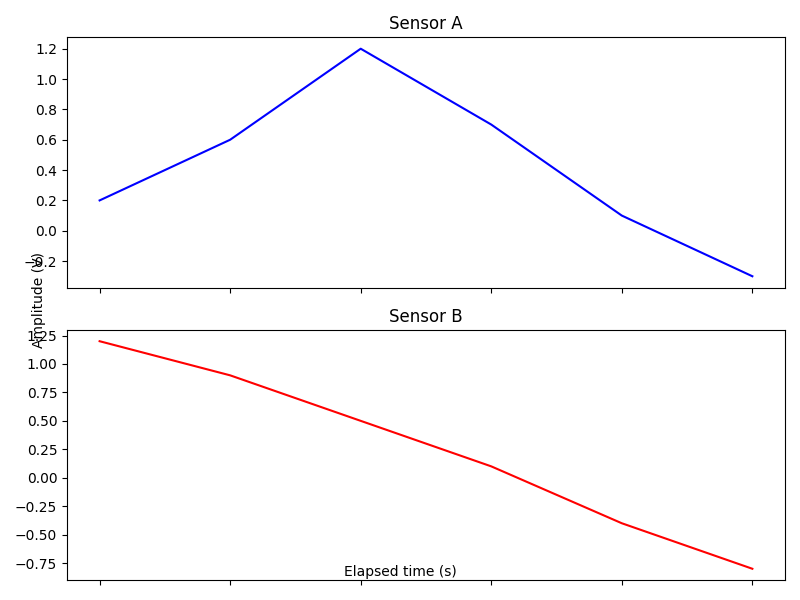
\includegraphics[width=0.80\linewidth]{runs/shared_axis_scope__ministral/figure.png}
\caption{Unmodified final artifact from
\texttt{shared\_axis\_scope\_\_ministral}.
The global x-label is inside the lower panel; the global y-label overlaps
numerical y ticks. Correct numerical values do not eliminate these
separate design and readability violations.}
\label{fig:authored-shared-min}
\end{figure}

\paragraph{Acceptable results and ambiguous boundaries.}
All five GLM runs, four other Ministral runs, and Qwen's temperature run
receive \texttt{[]}.
The numerical-task figures use $(145,0,95,105)$ USD for net revenue and
$(18.0,27.5,66.0,35.0)\%$ for monthly pooled rates.
Both channel figures use order counts $(120,75,210,45)$ and refund rates
$(4,8,3,6)\%$, with separate requested axis labels on both panels.
All three temperature figures retain six observations and convert their
times to $(0,1.5,3,4.5,6,7.5)$ minutes, with circular markers.

Several labeling boundaries matter.
The zero annotation in \path{filtered_net_revenue__glm} sits close above
the South tick name. The author reviewed the enlarged image and judged
both texts still distinguishable and readable. It is accepted as mild
crowding, not labeled \texttt{hard\_to\_read}.
In \path{pooled_success_rates__glm}, the blue line lightly contacts the
February annotation's percent sign, but the value $27.5\%$ remains legible;
this borderline contact is accepted as mild crowding, with the label
unchanged.
The temperature task expressly permits
\texttt{Temperature (C)} as well as \texttt{Temperature (degrees Celsius)};
different permitted unit wording is not an error.
Numeric x tick text is hidden in the Ministral shared-axis artifact, but
the prompt allows rather than requires such tick labels, so their absence
is not an extra violation.
Unrestricted colors, readable rotated category ticks, warnings, and an
unavailable auxiliary \texttt{file} command do not by themselves justify
an error. An intermediate incomplete image that is later overwritten does
not override the final artifact.

\paragraph{Observed label validation.}
The author ran:
\begin{verbatim}
uv run python -m workflow validate-labels
\end{verbatim}
and reported \texttt{valid: 15 human-reviewed label(s)}.
The checker establishes non-null entries, unique IDs, evidence fields,
execution-failure exclusivity, and exact run coverage.
Its wording alone does not certify personal human inspection; the
separate author review described above supplied that confirmation.

\subsection{Validator Performance on New Tasks}

\paragraph{Pre-iteration implementation and reproduction.}
The unchanged Part 2 validator was evaluated on the 15 authored runs,
using the same fixed validator model as before. Its source SHA-256 at this
checkpoint is:
\begin{verbatim}
7b968ed3ccccbcc9b2fa6fb0f69f314453913ace8b0c41e1a4649495a0627551
\end{verbatim}
The prediction file is
\path{output/pre_iteration_authored_predictions.json}.
The author ran the evaluation and subsequently the following scoring command:
\begin{verbatim}
uv run python -m validator.runner \
  --artifacts runs \
  --out output/pre_iteration_authored_predictions.json

uv run python -m workflow score \
  --predictions output/pre_iteration_authored_predictions.json
\end{verbatim}
The scorer uses \path{labels.json} by default.
The reported values below are the author's observed command output,
rounded to four decimal places.

\begin{table}[htbp]
\centering
\small
\begin{tabular}{lrrrrrrr}
\toprule
Error family & N & TP & TN & FP & FN & $+/-$ & MCC \\
\midrule
\texttt{execution\_failure} & 15 & 4 & 11 & 0 & 0 & 4/11 & $1.0000$ \\
\texttt{wrong\_data} & 11 & 0 & 6 & 5 & 0 & 0/11 & $0.0000$ \\
\texttt{wrong\_chart} & 11 & 0 & 10 & 0 & 1 & 1/10 & $0.0000$ \\
\texttt{hard\_to\_read} & 11 & 0 & 8 & 2 & 1 & 1/10 & $-0.1491$ \\
\bottomrule
\end{tabular}
\caption{Measured pre-iteration performance against the human-confirmed
reference labels. N is eligible run count; $+/-$ denotes positive/negative
reference support. Macro-MCC is \textbf{0.2127}.
The data family has insufficient positive reference support.}
\label{tab:authored-pre}
\end{table}

\paragraph{Support, scoring conventions, and scope.}
Execution is evaluated on all 15 records.
The four terminal reference execution failures are excluded from the
other three families, leaving 11 eligible examples in each.
No reference annotation names \texttt{wrong\_data}, so its zero MCC
reflects the assignment's insufficient-support convention, not perfect
data checking or an estimate of data-error recall.
The five data false alarms remain important measurable failures on correct
numerical transformations.
In contrast, \texttt{wrong\_chart} has both reference classes, but the
validator predicts no chart errors and misses the one positive; its MCC
is zero because predictions are constant-negative.
Readability has two false alarms and one missed positive, hence negative MCC.

Macro-MCC still averages all four families, including the
insufficient-support zero; it is not recomputed over only supported families.
The perfect execution score drives much of the $0.2127$ aggregate.
On this reference set, even perfect predictions in the other three supported
families would cap macro-MCC at $0.75$ under the data-support convention.
This is a property of this small set, not a ceiling on the private grading
set, which contains both reference classes for every family.
No additional reference error was invented to manufacture balanced support.

Part 3 specifies reporting and analyzing these outcomes, not a minimum
authored-set MCC. The five tasks are deliberately selected stress tests,
not a representative estimate of private-set performance.
The difference from the seed-set macro-MCC of $0.2411$ is not a measured
regression caused by a code change: the implementation is unchanged and
the task and label distributions differ.
Scores and error counts use the author's confirmed 15-run reference file.

\paragraph{Successes.}
All four missing-artifact runs are correctly reported as execution failures,
including the Qwen run whose outcome says \texttt{Submitted}.
This supports the artifact-delivery gate on these observed cases, without
claiming universal execution accuracy.
The five acceptable GLM runs all receive \texttt{[]}.
However, an empty prediction is not always correct: the genuinely flawed
Ministral shared-axis figure also receives \texttt{[]}.

\paragraph{Five data-family false positives.}
The exact false-positive runs are:
\path{filtered_net_revenue__ministral},
\path{panel_unit_labels__ministral},
\path{pooled_success_rates__ministral},
\path{semantic_unit_labels__ministral}, and
\path{semantic_unit_labels__qwen}.
Their explanations identify concrete validator weaknesses:
\begin{itemize}
\item For the filtered-revenue run, the explanation quotes
\texttt{Completed-order net revenue} on both sides but alleges a capitalization
difference. The requested and displayed titles are identical, and the four
net sums are correct. Even a genuine title mismatch would be a design issue,
not evidence that plotted numerical data is wrong.
\item For the channel run, the explanation alleges x-labels reading
\texttt{channel}; both actual panels visibly read \texttt{Sales channel}.
It also objects to the blue/green colors while acknowledging that colors
were unspecified. Correct plotted counts and refund rates are not invalidated
by these fabricated or out-of-family complaints.
\item For the pooled-rate run, the explanation lists the correct four
percentages and begins recomputing the correct ratios, without establishing
a discrepancy between requested and plotted values. The executed calculation,
final annotations, and independently derived targets agree.
\item For the Ministral temperature run, the explanation itself accepts the
axis labels, title, converted time, and circular-marker data, then describes
its remaining alleged concern as still acceptable. It nevertheless emits
\texttt{wrong\_data}, a decision/evidence contradiction.
\item For the Qwen temperature run, the explanation repeatedly acknowledges
the valid separate axis labels, correct conversion, and correct points.
Numeric tick labels need not each repeat the unit when a separate axis label
states it. This speculation does not establish a plotted-data error.
\end{itemize}

\paragraph{Readability false positives and missed errors.}
\path{pooled_success_rates__ministral} is incorrectly accused of overlapping
annotations and a y-label obscured by the title. In the final image the
percentage annotations are separated from their points and the y-label
is unobscured.
\path{semantic_unit_labels__qwen} is incorrectly accused of a partly clipped
\texttt{Temperature (C)} label; the complete label, including \texttt{(C)},
is visible.
These are two readability false positives.

Conversely, \path{shared_axis_scope__ministral} receives no errors despite
the misplaced shared x-label and overlapping shared y-label
(Figure~\ref{fig:authored-shared-min}).
It is therefore one false negative in each of the design and readability
families. The absence of intermediate design-audit outputs prevents
pinpointing the precise stage that missed the design violation.
Possible mechanisms include omitting relative placement from the checklist,
accepting the existence of \texttt{fig.text} without verifying its location,
or weak visual localization; these are hypotheses, not logged causes.

\paragraph{Agent failures versus validator failures.}
The Qwen action loops, invalid-column persistence, unsuccessful package-repair
attempts, and premature submission are failures of the visualization agents.
The delivered Ministral shared-label layout is another agent mistake.
By contrast, fabricated title/label differences, objections to unrestricted
colors, contradictory data judgments, imaginary clipping, and acceptance
of the genuine overlap are failures of the validator.
A recovered intermediate error must not be conflated with a failed final
artifact.

\paragraph{Mechanism motivating a subsequent improvement.}
The data and readability branches still use \path{validator/baseline.py}'s
broad YES/NO helper. It requests at most 250 output tokens and turns any
leading \texttt{YES} into an error of the selected family; it does not check
whether the explanation supports that decision or stays within that family.
This implementation and the observed contradictory positives motivate a
general improvement to structured decisions and evidence consistency,
rather than a task-ID-specific exception.

Some saved explanations end mid-sentence or mid-calculation, consistent with
an output-limit problem. However, the prediction file does not preserve
completion \texttt{finish\_reason}, so truncation and its causal effect
cannot be established from these predictions alone.
The chart-audit miss likewise cannot be attributed to a particular internal
stage without intermediate outputs.
No Part 4 validator change or targeted rescue call has been made at this
checkpoint.

\subsection{Harbor Packaging}

\paragraph{Completed staff worked example.}
Before packaging the authored tasks, the author ran the supplied Harbor
example under local Docker with the project's Harbor dependency.
Unlike the earlier model-based validator, this example uses a deterministic
pytest verifier. The \texttt{oracle} agent executes the task's reference
\path{solution/solve.sh}; \texttt{nop} performs no agent actions.
Neither invokes an LLM.

\begin{table}[htbp]
\centering
\small
\begin{tabular}{llrrr}
\toprule
Job & Answer under test & Reward & Exceptions & Time (s) \\
\midrule
\path{example-oracle} & Staff reference & $1.0$ & 0 & 30 \\
\path{example-nop} & No answer & $0.0$ & 0 & 10 \\
\path{example-illegible} & Staff unreadable mutant & $1.0$ & 0 & 11 \\
\bottomrule
\end{tabular}
\caption{Observed worked-example results, with one trial per job.
Times are the whole-second runtimes displayed by the CLI.
These are staff-example experiments, not rewards for the five authored
tasks or the two required self-authored mutants.}
\label{tab:harbor-worked-example}
\end{table}

The reference passes all 15 pytest checks. The no-op is rejected because
the required script and figure are absent.
Its pytest summary includes three failures, one pass, and 11 setup errors
from fixtures that cannot re-execute a missing plotting script.
These are expected verifier failures for an empty submission, not 11
Harbor infrastructure exceptions; the job reports zero exceptions.
The pair demonstrates that this example rewards its reference and
withholds reward from a no-answer submission.

\paragraph{Measured accepted-mutant limitation.}
For the required example-mutant experiment, the author copied the example
to a fresh temporary directory and replaced only that copy's reference
script with \path{harbor/example/mutants/illegible/solve.sh}.
The original staff reference remained unchanged.
The collected mutant script uses a $3\times2.2$ inch canvas at 100 DPI
and 2pt title, axis-label, and tick text. The saved $300\times220$ PNG has
extremely small text, a \texttt{hard\_to\_read} defect.
However, its orchard totals remain
$(558,420,1230,816)$ kg in the correct alphabetical order, and its
\texttt{plotted\_values.json} agrees with those numbers.

All 15 checks pass and the observed reward is $1.0$.
The checks establish artifact validity, input integrity, data and structural
properties, consistency with a fresh render, response to input perturbation,
and agreement of the sidecar. None evaluates rendered-text legibility.
Thus the accepted wrong answer measures an actual limitation, rather than
merely asserting that the verifier might miss something.
It motivates evaluating the rendered image as well as the declared numbers
and plot structure. It does not prove that a VLM would catch this particular
mutant: no VLM-validator call was made on this worked example.

\paragraph{Worked-example reproduction and retained evidence.}
The following commands reproduce the three experiments from the release root,
with Docker running. Fresh job names are needed when retaining earlier jobs.
\begin{verbatim}
uv run harbor run -p harbor/example \
  -a oracle --job-name example-oracle
uv run harbor run -p harbor/example \
  -a nop --job-name example-nop

hw2_mutant_dir=$(mktemp -d \
  /private/tmp/hw2-example-illegible.XXXXXX)
cp -R harbor/example/. "${hw2_mutant_dir:?}/"
cp harbor/example/mutants/illegible/solve.sh \
  "${hw2_mutant_dir:?}/solution/solve.sh"
uv run harbor run -p "${hw2_mutant_dir:?}" \
  -a oracle --job-name example-illegible
\end{verbatim}
The corresponding local evidence is in
\path{jobs/example-oracle/}, \path{jobs/example-nop/}, and
\path{jobs/example-illegible/}: each has a job \texttt{result.json}
and a trial's \path{verifier/reward.txt} and \path{verifier/pytest.log}.
The reference and mutant also retain the delivered figure, script, and
sidecar under the trial's \path{artifacts/app/} directory.
The report records the outcomes; these local job logs do not replace any
required submission artifacts.

\paragraph{Authored Harbor packages and measured reference rewards.}
All five authored task directories now have a completed Harbor instruction,
pinned offline environment, \texttt{task.toml}, reference script, and
task-specific deterministic checks. The added output contract asks for a
re-runnable \texttt{plot.py}, its \texttt{figure.png}, and a precisely typed
\texttt{plotted\_values.json}. Each verifier compares its sidecar with
independently derived literal answers. It checks the chart's data and
selected design requirements using a manifest captured during an isolated
replay of the plotting script, then compares the replayed PNG bytes and
sidecar with the delivered files. The original five task prompts and CSVs
are preserved.

\paragraph{Verifier-contract audit.}
A subsequent audit tightened agreement between the Harbor instructions and
their deterministic tests without changing the original tasks, generated
runs, human-confirmed labels, or pre-iteration validator. The added
\texttt{Required outputs} blocks now state the existing regular-file,
PNG-size/color, 60-second replay, and exact artifact-reproduction safeguards
explicitly. These basic validity guards do not certify visual readability.
The test implementation was also made less restrictive where the task
leaves a choice open: axis scales are not forced to be linear unless the
task requires it; correct bars may be created through multiple
\texttt{BarContainer} objects; a decorative zero-baseline line is allowed
without admitting an additional data series; and semantic unit labels use
Unicode NFKC normalization to recognize equivalent Celsius notation.
These are task-specific verifier robustness changes, not an additional
iteration of the general-purpose VLM validator; they do not change the
pre-iteration MCC scores. After the audit, all five references, both
mutants, and the do-nothing control were re-run in fresh Harbor jobs.
The rewards below were reconfirmed against this revised verifier, rather
than inferred from the earlier version's results.

\paragraph{Offline contract regression tests.}
\path{tests/test_harbor_verifier_contract.py} adds 20 deterministic tests
that capture actual Matplotlib artists in memory and invoke the packaged
checks. They exercise the newly accepted implementations and negative
controls for incorrect values, missing or extra bars, horizontal bars,
nonzero baselines, additional data series, wrong units, and mismatched
shared-axis scales. All 20 passed, and the full local suite passed all
122 tests. These tests do not call a model or replace the Docker replay
experiments. The suite can be reproduced from the release root with:
\begin{verbatim}
PYTHONDONTWRITEBYTECODE=1 .venv/bin/python -m unittest \
  discover -s tests -p 'test_*.py'
\end{verbatim}

Harbor 0.23.0 accepted each of the five packages in its preflight.
Each was then run once against its own reference solution using
\texttt{-a oracle}. The post-audit runs had one trial each, no
exceptions, and the rewards shown in Table~\ref{tab:authored-harbor}.
The recommended \texttt{-a nop} check on
\path{filtered_net_revenue} scored $0.0$ with zero exceptions.
Thus the verifier gives a completed reference full credit while denying
credit to an empty answer.

\begin{table}[htbp]
\centering
\small
\begin{tabular}{p{0.50\linewidth}rr}
\toprule
Authored task & Oracle reward & Exceptions \\
\midrule
\path{filtered_net_revenue} & $1.0$ & 0 \\
\path{panel_unit_labels} & $1.0$ & 0 \\
\path{pooled_success_rates} & $1.0$ & 0 \\
\path{semantic_unit_labels} & $1.0$ & 0 \\
\path{shared_axis_scope} & $1.0$ & 0 \\
\bottomrule
\end{tabular}
\caption{Five measured post-audit authored-task oracle runs. These are separate
from the staff worked-example runs in Table~\ref{tab:harbor-worked-example}.}
\label{tab:authored-harbor}
\end{table}

\paragraph{Two authored mutants and the measured verifier boundary.}
The two scripts under
\path{harbor/tasks/filtered_net_revenue/mutants/} were tested in
separate temporary copies of the task. Neither replaced the submitted
reference solution. The \path{ignore_status} mutant sums all orders,
including failed and pending rows. It plots $(345,225,140,105)$ rather
than the completed-only $(145,0,95,105)$ for North, South, East, and
West. Its observed reward was $0.0$, with zero Harbor exceptions.
The pytest log names
\path{test_sidecar_net_revenue_matches_expected} as a failing test;
the literal sidecar comparison reports
\texttt{North: expected 145, got 345.0}. The plotted-bar value and
required-annotation tests also fail, so the rejection is grounded in
the answer's wrong data rather than an infrastructure error.

The \path{illegible} mutant applies the correct completed-only
calculation and preserves the required labels and numbers, but uses
2pt text on a $300\times220$ PNG. Inspection of the saved PNG shows
that the text is too small to read at its delivered size, a
\texttt{hard\_to\_read} error. It nevertheless passed all four pytest
checks: observed reward $1.0$ and zero exceptions. This is a measured
limitation of the authored deterministic verifier. It checks that text
exists, but does not measure rendered font size, overlap, or contrast.
The worked-example mutant above is separate and does not count as
either of these two authored mutants.

\paragraph{Reproduction and retained evidence.}
The following commands illustrate the authored checks from the release
root. Use fresh job names if retaining the existing results.
\begin{verbatim}
for id in filtered_net_revenue panel_unit_labels \
          pooled_success_rates semantic_unit_labels \
          shared_axis_scope; do
  uv run python harbor/preflight.py "harbor/tasks/$id"
  uv run harbor run -p "harbor/tasks/$id" \
    -a oracle --job-name "$id-oracle-contract-audit"
done

for mutant in ignore_status illegible; do
  trial_dir=$(mktemp -d /private/tmp/hw2-"$mutant".XXXXXX)
  cp -R harbor/tasks/filtered_net_revenue/. "$trial_dir/"
  cp "harbor/tasks/filtered_net_revenue/mutants/$mutant/solve.sh" \
    "$trial_dir/solution/solve.sh"
  uv run harbor run -p "$trial_dir" -a oracle \
    --job-name "filtered_net_revenue-$mutant-contract-audit"
done

uv run harbor run -p harbor/tasks/filtered_net_revenue \
  -a nop --job-name filtered_net_revenue-nop-contract-audit
\end{verbatim}
The observed jobs are retained locally under \path{jobs/}, in:
\begin{verbatim}
<task_id>-oracle-contract-audit/
filtered_net_revenue-ignore_status-contract-audit/
filtered_net_revenue-illegible-contract-audit/
filtered_net_revenue-nop-contract-audit/
\end{verbatim}
Their trial
directories contain \path{verifier/reward.txt} and
\path{verifier/pytest.log}. The job directories are development logs
and are not required submission artifacts.

The deterministic verifier can identify an execution failure in the
specific sense that required files are missing, invalid, or not reproduced
by the saved script. Its literal calculations and captured plot values can
identify many \texttt{wrong\_data} cases for these five known tasks.
Captured artist types, labels, panel arrangement, and axis relationships
cover some \texttt{wrong\_chart} cases. They do not certify every spatial
detail of annotations or labels. The PNG validity check cannot decide
\texttt{hard\_to\_read}; a visually illegible but structurally correct
plot can pass. The verifier also does not prove that a submission derived
its values from the CSV rather than hard-coding the correct answer.
The two measured authored mutants show one successful numerical check
and one missed readability defect.

A per-task verifier has the answer key and output schema for its own
task. The validator evaluated on private runs receives unseen prompts
and trajectories without an independent answer key, so these authored
checks cannot replace that validator.

After completing the Part 4 predictions, report, and AI-usage declaration,
the author ran the complete end-to-end \texttt{check-submission} command.
Its observed results are recorded in
Section~\ref{sec:final-submission-verification}.

\section{Part 4: Iterate on Your Design}

\subsection{Additional Improvement Motivated by Part 3}

\paragraph{Observed motivation, not a new answer key.}
Part 3 exposed five \texttt{wrong\_data} false positives on numerically
correct authored figures and two \texttt{hard\_to\_read} false positives
on legible figures (Table~\ref{tab:authored-pre}).
For example, \path{filtered_net_revenue__ministral} was accused of a
title difference even though the quoted titles were identical, and
\path{pooled_success_rates__ministral} was flagged while its explanation
recomputed the correct pooled rates. These are respectively an
out-of-family complaint and a decision/evidence contradiction.
The readability branch imagined annotation overlap on that pooled-rate
figure and clipping on \path{semantic_unit_labels__qwen}, while missing
the actual shared-y-label overlap in
\path{shared_axis_scope__ministral}.
The latter run also remains an important \texttt{wrong\_chart} false
negative: this iteration changes the data and readability branches, not
the existing chart-design audit.

The common mechanism targeted here is the baseline helper's conversion
of a leading \texttt{YES} into a family error without checking its
supporting explanation. I replace that helper in both branches with
family-specific structured coverage, strict response validation, and a
bounded same-model reinspection of provisional errors or uncertainty.
This is a general evidence-consistency change, not a rule keyed to the
five tasks, their run IDs, or their human labels.

\paragraph{Data audit: four explicit failure modes.}
The data branch receives the requested task, input-file contents,
executed trajectory, and final figure through the existing evidence
transport. It asks the fixed model to independently compare the
requested and delivered data across exactly four modes:
\texttt{wrong\_values}, \texttt{missing\_data},
\texttt{wrong\_selection}, and \texttt{wrong\_order}.
The current response object has these four mode names as its fixed
top-level keys, with no extras or omissions. Each mode contains exactly
\texttt{status}, \texttt{evidence}, and \texttt{finding}.
Status is \texttt{pass}, \texttt{fail}, or \texttt{uncertain}; evidence
is a nonempty string of at most 160 characters. A mode with no applicable
constraint still requires an explanatory pass check.
The policy covers derived values, normalization, sampling ranges,
data-encoded sizes/colors/error bars, missing dimensions, filters,
extra unrequested series, and requested ordering. It explicitly separates
these from title/axis-label wording, arbitrary styling, and readability.
An intermediate broken command repaired before the delivered figure is
not by itself a final data defect.

For a failed mode, its \texttt{finding} is one object containing only
\texttt{source\_id}, \texttt{location} (at most 80 characters),
\texttt{expected}, and \texttt{observed} (at most 160 characters each).
For pass/uncertain modes, \texttt{finding} must be JSON \texttt{null}.
The model therefore does not repeat the mode name, task quotation, or
evidence in a separate findings array. Internally, the program converts
this compact response into the shared canonical checks/findings
representation. The earlier two-array format remains a historical
implementation choice at the first two checkpoints described below.
The program assigns canonical IDs to the original nonempty task lines;
the model selects an ID, and the program restores the corresponding
source text rather than trusting a rewritten quotation.
That source establishes the requested constraint, not the truth of the
claimed discrepancy. The model must still compare concrete final values,
selection, coverage, or ordering against the request.
An alleged failure whose expected/observed descriptions are identical
after whitespace normalization is not accepted as a confirmed defect.
Unlike the earlier format-rejection behavior, the current compact parser
turns that unsupported claim into provisional semantic uncertainty,
retaining it for the single evidence reinspection. It does not infer
that the data is correct or invent a discrepancy to repair the claim.
The policy also states that
numerically equal forms such as \texttt{27.5} and \texttt{27.50} are not
errors; this broader numerical interpretation remains model-based,
not a general symbolic or numerical equivalence proof by the parser.
Final executed calculations, when available, are preferred to approximate
numerical readings from pixels. A projection mistake alone does not
establish that a requested data dimension is missing. Colormap choice,
axis scales, title text, and marker styling are not data defects merely
because they violate a design requirement; an actual error in the data
encoding or values must be established separately.

\paragraph{Readability audit: final pixels, six explicit modes.}
The readability branch now inspects the original delivered PNG with
task text as context, without CSV contents or the execution trajectory.
This isolates visible readability from numerical correctness and from
what plotting code claims to have drawn. Exactly one check is required
for each of \texttt{clipped\_text}, \texttt{overlapping\_text},
\texttt{occlusion}, \texttt{low\_contrast},
\texttt{indistinguishable\_data}, and \texttt{squeezed\_layout}.
A failed mode needs a localized finding naming the affected
\texttt{location}, \texttt{elements}, visible \texttt{observation}, and
reading \texttt{impact}, in addition to its \texttt{kind}.
The policy distinguishes partial clipping from an entirely missing
required label, and actual overlap or occlusion from harmless proximity
or a legend over empty space. Numeric ticks need not repeat units already
given by an axis label. A visible low-contrast label is not simply
treated as an absent design element.

Readability requests always retain the original PNG bytes; this branch
does not resize the image to solve a context error and then mistake
downsampling artifacts for defects in the delivered output.
If the endpoint rejects the request for context length, it retries once
without task text while preserving that original image. The omission
is explicitly marked and cannot establish a missing requirement.
If the image-only request still cannot fit, the operational error is
propagated. In contrast, the data branch retains the existing evidence
compaction transport from Part 2, including marked input/trajectory
omissions and its in-memory image reduction when necessary. A compacted
data judgment therefore retains the earlier evidence-loss limitation.

\paragraph{Deterministic validation versus semantic confirmation.}
Both branches request strict JSON schemas. Data uses the four-key compact
format above; readability retains exactly \texttt{checks} and
\texttt{findings}. Local parsing rejects duplicate JSON keys, unknown or
missing fields, non-string or empty evidence, incomplete/duplicate
coverage, invalid statuses, and invalid failure/finding correspondence.
Data string bounds are stated with JSON Schema \texttt{minLength} and
\texttt{maxLength} and also checked locally; this does not demonstrate
that every live response will succeed. Data source IDs must belong
to the supplied task-line map, and pass/uncertain modes must carry null
findings. Readability failures retain exactly one localized finding per
failed mode and none for pass/uncertain modes. These are structural and
consistency checks. They do not prove that a model observed the right
pixel, recomputed a formula correctly, or interpreted a requirement
faithfully. A false explanation can still satisfy the schema.

A valid all-pass response is returned without a confirmation call.
If a check fails or is uncertain, each branch performs one grouped
same-model reinspection against the original evidence and explicitly
fallible provisional claims. Data requests all four compact-mode checks
again; readability requests its full six-mode coverage. The model may
revise those checks rather than being forced to preserve an earlier
verdict. Both use the same fixed model, not an independent judge or a
calibrated confidence estimate; correlated errors can persist.
The selected final implementation does not use the additional three-gate
support-review experiment documented under Further Changes below.

Each response stage allows at most two format attempts: an initial
attempt and one repair after invalid JSON, inconsistent fields, or a
completion with \texttt{finish\_reason=length}. There is at most one
semantic reinspection stage per family in a validator invocation;
there is no open-ended loop until a preferred answer appears.
In the current data policy, semantic uncertainty that persists after
valid JSON and that one reinspection produces a \texttt{RuntimeWarning}
and withholds an unconfirmed \texttt{wrong\_data} allegation. The public
binary output has no uncertainty category, so the result is absence of
that data-family error, not proof of data correctness. This is an
explicit conservative classification policy: it may suppress false
positives and avoid aborting a run over an unsupported model claim,
but may introduce false negatives. It is not merely a transport fix,
an automatic pass for malformed replies, or completion of missing labels.
Malformed/truncated JSON, missing evidence, invalid source IDs, or invalid
null/finding coupling still raise operational errors after bounded format
repair. Interface/network exceptions propagate rather than being repaired
as response-format errors or withheld as semantic uncertainty.
Readability and chart-audit uncertainty
retain their earlier operational-error behavior. A confirmed failure
can still be returned while another mode remains uncertain, because the
demonstrated finding already establishes that family. Context retries
and the unchanged runner's operational retries are distinct from this
semantic bound.

The regular data and readability completion budgets are respectively
1,536 and 2,048 tokens, replacing the baseline helper's 250-token limit
for those two branches. Both an initial data judgment and its optional
semantic reinspection start at 1,536 tokens. Following the incomplete
first seed experiment described below, a data response explicitly ending
with \texttt{finish\_reason=length} receives its one format-repair
attempt with a bounded 3,072-token budget. Non-length format problems
do not trigger that increase; readability remains at 2,048 tokens.
This provides space for four/six coverage checks and specific findings;
it does not establish that the old saved baseline answers were truncated,
nor guarantee that a new response fits.
Malformed or length-limited new responses are detected directly instead
of accepted merely because their first word is \texttt{YES}.
The output remains the prescribed list of \texttt{Error} objects;
multiple confirmed findings of one family are combined into its evidence.

\paragraph{Preserved controls and expected tradeoffs.}
The Part 2 execution gate and scoped chart-design audit are unchanged.
All calls still use \path{Qwen/Qwen3-VL-30B-A3B-Instruct-FP8};
no alternate model, reference image, label file, or cross-run answer is
consulted by \texttt{validate(run)}. The function signature and public
prediction schema are unchanged. The five original task prompts,
15 agent runs, and confirmed reference labels are held fixed.
The separate pre-iteration prediction files remain the before-change
comparators: seed macro-MCC $0.2411$ and authored macro-MCC $0.2127$.

\paragraph{Initial implementation checkpoint and offline verification.}
The first Part 4 implementation checkpoint had SHA-256:
\begin{quote}
\small
\path{f818fae884b79c981e0a53b7d97ba554c6ad45e0028cba5abc8b6514824b6a48}
\end{quote}
At this checkpoint, all 175 local regression tests passed, including
53 new data/readability tests in \path{tests/test_solution_evidence.py}.
The full suite can be reproduced from the repository root with:
\begin{verbatim}
PYTHONWARNINGS=ignore::DeprecationWarning \
PYTHONDONTWRITEBYTECODE=1 \
.venv/bin/python -m unittest discover -s tests -p 'test_*.py'
\end{verbatim}
The synthetic-response tests checked schema/coverage invariants, bounded
repair/reinspection, operational-error propagation, and original-PNG
readability transport. They established implementation mechanics, not
live judgment accuracy or MCC improvement. This identifies the initial
source, not a later revision or completed final experiment.

\paragraph{Observed operational failures and bounded robustness revision.}
The first seed evaluation using that checkpoint produced 104 of the
required 110 predictions. The omitted run IDs were
\texttt{009}, \texttt{106}, \texttt{117}, \texttt{164},
\texttt{177}, and \texttt{205}. They are missing validator outputs,
not six new reference \texttt{execution\_failure} labels.
The recorded terminal validation problems identify four length-limited
data responses (009, 117, 177, and 205), an identical expected/observed
claim (106), and duplicated or orphaned findings (164).
The original raw failed judge responses were not stored, and the old
terminal errors did not distinguish initial judgment from semantic
confirmation. Consequently, the failed stage and the full content of
each rejected answer cannot be reconstructed from that record.
The incomplete prediction snapshot is preserved separately in
\path{tests/diagnostics/part4_seed_incomplete_f818fae8.json}; it must not
be presented as the final complete seed prediction file.

That first revision retained strict parsing, added the length-triggered
3,072-token data repair budget, and supplied targeted repair instructions
for identical comparisons and orphaned/duplicate findings. They asked
the model to re-evaluate the original evidence, never invent a discrepancy,
and synchronize one finding per real failed mode. Attempt/reinspection
bounds were unchanged. Terminal diagnostics added the initial/confirmation
stage, \texttt{finish\_reason}, output budget, and response character count
without raw content. These are general response rules, not public-ID
exceptions; the probe below measures their limited live effect.

\paragraph{First robustness checkpoint and measured repair probe.}
The first robustness revision had SHA-256:
\begin{quote}
\small
\path{0649b1409575cf4ee543a0e0a5869a5006f5168a09e89fc40a9a0db71d6a976a}
\end{quote}
At this checkpoint, the full local suite passed all 200 tests, including
25 additional offline repair regressions in
\path{tests/test_solution_repair.py}. The command above reproduces the
suite. These synthetic-response tests cover truncation-only budget
growth, independent initial/confirmation budgets, actual last-attempt
diagnostics, strict contradiction/finding rejection, bounded attempts,
unchanged readability budget, and original-evidence retention. They do
not by themselves establish successful live completion.
The author then ran a separate six-record repair probe using this source.
Its preserved output,
\path{tests/diagnostics/part4_repair_probe_0649b140.json}, contains
four completed predictions: 106, 117, 164, and 205.
Run 117 eventually succeeded after earlier attempts failed;
009 and 177 remained missing. Across the runner's passes, 009 again
reported length termination in the initial data stage despite the
3,072-token repair budget (the reported last response length was
6,421 characters). Run 177 reported finding-correspondence and identical
comparison problems in initial or confirmation stages.
The probe demonstrates four completed evaluations, not four correct
classifications. In particular, 106 still assigned \texttt{wrong\_data}
to a requested-versus-observed colormap difference, which is a design
violation rather than an established numerical/data discrepancy.
This exposes continuing family leakage even when strict JSON parses.
The six-record probe is not a complete seed/authored scoring experiment;
no overall final MCC or measured runtime improvement is claimed from it.

\paragraph{Selected final compact-data revision and uncertainty policy.}
The remaining verbosity and parallel-array synchronization failures
motivated the compact four-key response described above. Bounded strings
and nonrepeated findings reduce response redundancy without removing
any of the four data modes. The same-value rule now treats an unsupported
but structurally complete comparison as uncertainty for one reinspection,
instead of repeatedly demanding a format correction for a semantic
contradiction. The final uncertainty-withholding policy is documented
explicitly above because it changes classification behavior and can
reduce recall; it cannot be presented as a purely technical fix.
Family-boundary guidance is also strengthened in response to the probe's
colormap allegation. The normal budgets, two format attempts, one
semantic review, fixed model, and execution/design/readability mechanisms
remain unchanged. The six-record probe below measures live completion,
and the complete seed result appears in the final-evaluation subsection.
After rejecting the further experiment described below, I restored this
exact source, not a modified variant. Its complete seed predictions
therefore remain applicable without rerunning 110 records; the final
authored evaluation must use this same frozen source. Resuming into a
file from a different source would invalidate attribution.

The selected final validator has SHA-256:
\begin{quote}
\small
\path{f7ff977319d330c9ac78e59205cd6d745a35a1d100d770d3d5700a0e963bd2de}
\end{quote}
All 223 offline tests passed at this checkpoint, including 23 new compact
protocol regressions in \path{tests/test_solution_compact_data.py}.
After restoring the exact selected source and its fixtures, the active
223-test suite was rerun and passed again.
The existing data/readability integration fixtures were adapted to the
new wire format; direct tests of canonical parsing and bounded repair
were retained. The new tests cover fixed-key coverage, field-length and
null/status constraints, task-source grounding, duplicate-key rejection,
same-value claims becoming uncertainty rather than proven correctness,
bounded reinspection, warning/withholding of unresolved semantic claims,
preservation of other supported findings, and propagation of malformed,
truncated, and interface failures. These tests use synthetic model
responses and establish code behavior, not live completion, speed, or
semantic accuracy. Both complete final evaluations are reported below.

\paragraph{Measured compact-protocol probe and remaining limitations.}
The author reran the same six previously omitted seed runs using the
compact checkpoint and a separate prediction file,
\path{tests/diagnostics/part4_compact_probe_predictions.json}.
The file validates against the prescribed prediction schema and contains
exactly one prediction for each of 009, 106, 117, 164, 177, and 205, with
nonempty evidence and no duplicate error families. All six completed in
the first runner sweep; the displayed sweep time was 7 minutes 50 seconds.
This is not a controlled latency comparison: per-stage format attempts,
serving state, and token usage were not recorded. The console emitted a
semantic \texttt{missing\_data} uncertainty warning for 106 after the one
reinspection. Its final output reports only \texttt{wrong\_chart}; withholding
that unconfirmed data allegation does not prove the data correct.

Completion is distinct from semantic correctness. Against the provided
reference labels on these six records only, data has two true positives,
one true negative, and three false positives (009, 177, and 205), with no
false negatives. Readability has two true positives, one true negative,
two false positives (117 and 164), and one false negative (177).
For example, 009's final executed script contains and plots all 23 requested
version/date pairs, but the validator alleges missing and extra versions.
On 177 it invents a required exact panel title and treats a pie-to-bar
design mismatch as a data defect. On 117 an actual omitted data dimension
supports a positive data-family label, but another supporting finding
still alleges a spelling difference between the identical title word
\texttt{Rossler} and itself; structural validation does not prove every
clause of a comparison. Thus a family-level true positive need not have
wholly correct evidence. This selected six-record diagnostic resolves the
observed completion failures in that run, not all classification or evidence
errors. It is not substituted for either required full-set evaluation,
and no complete-set MCC improvement is inferred from it.

The initial aim was to reduce false data/readability allegations and
better localize actual overlap. The complete seed experiment measures
an aggregate improvement, but does not establish improved data precision:
the data false-positive count increased substantially. Full coverage
and reinspection may also increase runtime and model cost; same-model
confirmation can retain correlated errors. In particular, the small
authored set has no positive \texttt{wrong\_data} reference examples,
so even eliminating its data false positives cannot establish data-error
recall or change that family's insufficient-support MCC convention.
The full seed results below belong to the selected final compact source,
not to the rejected support-review experiment. The authored comparison
and case-level FP/FN analysis are also reported below.

\subsection{Final Evaluation on Seed and New Tasks}
\paragraph{Incomplete first seed run: diagnostic only.}
For transparency, Table~\ref{tab:part4-incomplete-diagnostic} compares
the initial Part 4 predictions with the preserved Part 2 predictions
on their common 104 run IDs. This is an offline diagnostic calculation,
not a completed invocation of the assignment's final scoring workflow.
Both columns use identical IDs and the official reference eligibility
mask: all 104 records enter execution scoring, while the 12 terminal
reference execution failures are excluded from each other family,
leaving 92 eligible records there. No missing prediction is filled with
\texttt{[]} or a fabricated execution error.
\begin{table}[htbp]
\centering
\small
\begin{tabular}{lrr}
\toprule
Metric & Part 2, same 104 IDs & Initial Part 4, incomplete \\
\midrule
\texttt{execution\_failure} & $1.0000$ & $1.0000$ \\
\texttt{wrong\_data} & $-0.1455$ & $0.3263$ \\
\texttt{wrong\_chart} & $0.3377$ & $0.3103$ \\
\texttt{hard\_to\_read} & $-0.2474$ & $0.2293$ \\
Macro-MCC & $0.2362$ & $0.4665$ \\
\bottomrule
\end{tabular}
\caption{Matched-subset diagnostic for the first incomplete Part 4 seed
attempt. These are not the required full 110-run final scores, and they
do not measure the subsequent robustness revision.}
\label{tab:part4-incomplete-diagnostic}
\end{table}
The data/readability increase and chart decrease describe these matched
records only. In particular, the chart audit's implementation did not
change; model judgments can still vary between evaluation calls.
The six unresolved records prevent treating this subset as an unbiased
estimate of complete performance.

\paragraph{Complete seed evaluation of the selected final validator.}
The author evaluated the exact selected compact source on all 110 seed
records. Its source and full predictions are retained as
\path{tests/diagnostics/solution_compact_f7ff9773.py} and
\path{tests/diagnostics/part4_compact_seed_f7ff9773.json}.
The required \path{output/final_seed_predictions.json} is byte-identical
to that complete prediction snapshot.
The source has the \texttt{f7ff9773} hash reported above, and the snapshot
contains exactly the seed IDs with valid prediction objects. The values
in Table~\ref{tab:part4-compact-full} were checked read-only with the
official scorer function and then confirmed by the author's final
\texttt{workflow score} command. Restoring the exact same source
preserves this complete experiment rather than mixing implementations
or filling missing predictions by hand.
Execution uses all 110 records; the 12 terminal reference execution
failures are excluded from the other families, leaving 98 each.

\begin{table}[htbp]
\centering
\small
\begin{tabular}{lrrrrrr}
\toprule
Family & Part 2 MCC & Final seed MCC & TP & TN & FP & FN \\
\midrule
\texttt{execution\_failure} & $1.0000$ & $1.0000$ & 12 & 98 & 0 & 0 \\
\texttt{wrong\_data} & $-0.1445$ & $0.1802$ & 23 & 18 & 55 & 2 \\
\texttt{wrong\_chart} & $0.3512$ & $0.3849$ & 41 & 23 & 4 & 30 \\
\texttt{hard\_to\_read} & $-0.2424$ & $0.2197$ & 15 & 48 & 11 & 24 \\
\midrule
Macro-MCC & $0.2411$ & $0.4462$ & & & & \\
\bottomrule
\end{tabular}
\caption{Complete seed evaluation of the selected final compact-data
validator. Confusion counts are for that implementation; the baseline
seed macro-MCC was $0.0268$.}
\label{tab:part4-compact-full}
\end{table}

Aggregate improvement does not imply that the observed data false-alarm
problem was solved. Data false positives increased from 15 in Part 2 to
55, while false negatives decreased from 23 to 2; the compact version
became much more positive on that family. Its $0.1802$ MCC therefore
cannot be used as evidence of improved data precision. These full-set
results motivated the further three-gate experiment described below,
which was subsequently rejected rather than silently presented as final.
The before/after chart scores also vary although that branch's code is
unchanged, so their difference is not attributable to a chart-audit
implementation change. The authored comparison below uses the original
15 runs and unchanged reference labels, not regenerated runs or revised
labels selected to favor the final validator.

The standard end-to-end reproduction commands for the selected source are:
\begin{verbatim}
uv run python -m validator.runner \
  --artifacts artifacts \
  --out output/final_seed_predictions.json
uv run python -m validator.runner \
  --artifacts runs \
  --out output/authored_predictions.json
uv run python -m workflow score \
  --labels seed_labels.json \
  --predictions output/final_seed_predictions.json
uv run python -m workflow score \
  --predictions output/authored_predictions.json
\end{verbatim}
The seed evaluation was retained under the exact restored source;
the authored evaluation then used that same source, and the author ran
both final scoring commands. No mixed-source prediction file was assembled.

\paragraph{Complete final authored evaluation.}
The final \path{output/authored_predictions.json} contains exactly one
valid prediction for every one of the 15 authored run IDs, with no
missing or duplicate records. Its SHA-256 is:
\begin{quote}
\small
\path{0e39fe0f5255acf6de65c023b8fc44b125b61cbe192b802c4112653dc41ece49}
\end{quote}
The unchanged \texttt{f7ff9773} final source is the same one used for
the complete seed evaluation. Before-change authored predictions are
the preserved \path{output/pre_iteration_authored_predictions.json},
not regenerated answers from the final code.
Table~\ref{tab:part4-authored-final} reproduces the author's official
score output and gives the separate authored before/after comparison.

\begin{table}[htbp]
\centering
\small
\begin{tabular}{lrrrrrrr}
\toprule
Family & Before MCC & Final MCC & TP & TN & FP & FN & $+/-$ \\
\midrule
\texttt{execution\_failure} & $1.0000$ & $1.0000$ & 4 & 11 & 0 & 0 & 4/11 \\
\texttt{wrong\_data} & $0.0000$ & $0.0000$ & 0 & 7 & 4 & 0 & 0/11 \\
\texttt{wrong\_chart} & $0.0000$ & $0.0000$ & 0 & 10 & 0 & 1 & 1/10 \\
\texttt{hard\_to\_read} & $-0.1491$ & $1.0000$ & 1 & 10 & 0 & 0 & 1/10 \\
\midrule
Macro-MCC & $0.2127$ & $0.5000$ & & & & & \\
\bottomrule
\end{tabular}
\caption{Final authored performance against the unchanged, human-confirmed
15-run reference labels. Counts and $+/-$ support are for the final
validator. Execution is eligible on 15 records; the other families are
eligible on 11 after excluding four terminal reference execution failures.}
\label{tab:part4-authored-final}
\end{table}

The data family still has no positive reference support, so its MCC is
zero by convention before and after; this cannot establish data-error
recall. Nevertheless its false-positive count decreases from five to
four. Three old data false alarms disappear, two persist, and two new
ones appear, as detailed below. Chart design still predicts no positive
cases and misses the single reference positive, so its supported-class
MCC remains zero. Readability changes from TP/TN/FP/FN $0/8/2/1$ to
$1/10/0/0$, removing two false alarms and detecting the one positive.
This produces the authored macro-MCC increase from $0.2127$ to $0.5000$.
The perfect readability score has only one positive example and does
not certify general readability accuracy or explanation quality.

\subsection{Qualitative Analysis of Self-Authored Tasks}

\paragraph{Observed improvements and remaining data regressions.}
The final validator removes the pre-iteration data false positives on
\path{panel_unit_labels__ministral},
\path{semantic_unit_labels__ministral}, and
\path{semantic_unit_labels__qwen}.
The actual counts, semantic unit labels, converted times, and requested
data points in those figures are correct. The two persistent data false
positives are \path{filtered_net_revenue__ministral} and
\path{pooled_success_rates__ministral}; their final evidence now makes
incorrect numerical claims rather than merely repeating the earlier
label/style complaints. The new data false positives are
\path{filtered_net_revenue__glm} and
\path{shared_axis_scope__ministral}.
Thus lower total FP count does not mean that every data judgment or
the proposed family-separation mechanism succeeded.

\paragraph{Specific false positive: invented expected arithmetic.}
For \path{filtered_net_revenue__ministral}, the final explanation says
\texttt{Expected: 165. Observed: 145} and attributes the expected value
to gross $120+60$ and refunds $20+15$.
Those very numbers give $(120-20)+(60-15)=145$, not 165.
The final successful script was written in trajectory message index 8
and executed at index 10 (zero-based indexing). Its exact calculation
and aggregation lines are:
\begin{quote}
\small\ttfamily\raggedright
\noindent\detokenize{completed_orders.loc[:, 'net_revenue'] = completed_orders['gross'] - completed_orders['refund']}\par
\noindent\detokenize{net_revenue_by_region = completed_orders.groupby('region')['net_revenue'].sum()}
\end{quote}
The script filters exactly completed rows and reindexes all four regions;
the delivered North bar is correctly annotated 145. This is a definite
final \texttt{wrong\_data} false positive, supported by independent
arithmetic, task data, the executed script, and image. A plausible cause
is model arithmetic hallucination despite the structured evidence
format; the parser validates fields and literal consistency, not sums.
It cannot distinguish a plausible-looking expected value from a correct
one. The same limitation is visible in
\path{pooled_success_rates__ministral}: its final explanation calls
March's correct $66.0\%$ wrong and asserts $60.0\%$ instead.
The actual pooled calculation is
$100(27+6)/(30+20)=66.0\%$.
The executed script at message index 4 contains:
\begin{quote}
\small
\begin{verbatim}
lambda x: 100 * x['successes'].sum() / x['attempts'].sum()
\end{verbatim}
\end{quote}
Neither final allegation is justified by the plotted data.

\paragraph{New false positive: a zero-height category is not absent.}
For \path{filtered_net_revenue__glm}, final evidence says South is
missing and therefore also alleges wrong order/selection.
The final script at message index 6 explicitly includes the category:
\begin{quote}
\small
\begin{verbatim}
regions = ['North', 'South', 'East', 'West']
net_revenue = {region: 0 for region in regions}
\end{verbatim}
\end{quote}
It passes all four resulting values to \texttt{ax.bar}; the saved image
has the South tick and a zero annotation. A zero-height bar has no
positive-area rectangle to see, but its category is represented exactly
as requested. The likely weakness is confusing visually absent area
with absent data and failing to reconcile pixels with executed values.
That is a hypothesis about the judgment, not a logged internal cause.

\paragraph{Specific false negative: shared-label placement still missed.}
\path{shared_axis_scope__ministral} remains the authored
\texttt{wrong\_chart} false negative. The task requires the figure-level
x-label beneath the pair of panels and the y-label alongside the pair.
The repaired final script at trajectory message index 10, executed at
index 12, contains these exact lines:
\begin{quote}
\small
\begin{verbatim}
fig.text(0.5, 0.04, 'Elapsed time (s)', ha='center')
fig.text(0.04, 0.5, 'Amplitude (V)', va='center', rotation='vertical')
plt.tight_layout()
\end{verbatim}
\end{quote}
The source lines above omit only their trailing comments.
In the final pixels (Figure~\ref{fig:authored-shared-min}), the x-label
is inside the lower plotting area, above its bottom spine, rather than
below the panel pair. The shared y-label also overlaps the left ticks.
The final validator returns no \texttt{wrong\_chart} despite the location
violation. A plausible explanation is accepting the existence of
\texttt{fig.text} without checking the label's required position relative
to the saved panels, or weak visual localization. Intermediate checklist
and audit responses are not preserved in the prediction file, so no
particular internal cause is asserted as proven.

That run also becomes a new data false positive: the explanation objects
to missing per-panel labels, although the task explicitly requires
shared figure-level labels and forbids separate per-panel labels.
Its two numerical series are correct. This is an out-of-family
data allegation and a failure to preserve task scope, not evidence
that the plotted sensor data is wrong.

\paragraph{Readability improves at family level, not fully in evidence.}
The former readability false positives on
\path{pooled_success_rates__ministral} and
\path{semantic_unit_labels__qwen} disappear.
The shared-axis Ministral run is now a readability true positive, which
accounts for the final family's TP=1 and perfect MCC on this small set.
However, its explanation alleges that the x-label is cut off at the
image's right edge. The full x-label is actually visible near the bottom
center; the actual readability defect is the shared y-label's left-side
tick overlap. The misplaced shared x-label is a separate chart-design
violation, not partially clipped text. Therefore the correct family-level
prediction does not show that the new localization policy correctly
identified the true overlap mechanism. Its stated clipping evidence
is not supported by the saved image. This distinction matters because
the assignment assesses explanatory evidence separately from MCC.

\paragraph{Interpretation and generalization limits.}
The final authored results improve macro-MCC and readability
classification, but leave the chart-design miss and four data false
alarms. Seed macro-MCC also improves to $0.4462$, while its data false
positives rise from 15 to 55. The structured checks are therefore not
a general guarantee against unsupported positive judgments.
These are observed comparisons on fixed runs and labels, not controlled
ablations establishing which prompt, budget, reinspection, or context
change caused each difference. Same-model variation can affect even
unchanged branches. The small authored distribution has no positive
data reference cases and only one positive case each for chart design
and readability; it cannot estimate performance on the private task
distribution. No run-ID exceptions or reference-label lookups were added
to obtain these outcomes.

\subsection{Further Changes}
The first robustness revision added length-triggered adaptive repair,
targeted contradiction/finding repair, and stage-specific diagnostics.
Its measured six-record probe completed four records but still exposed
two operational failures and a colormap family leak. The compact revision
adds compact data output, stronger category boundaries, provisional
uncertainty for same-value claims, and explicit withholding of semantic
data allegations that remain unconfirmed after one review. The last
policy carries a false-negative risk. Neither revision modifies the five original
tasks, reference labels, or execution/design branches. Their motivations
are observed completion and evidence failures, not a desired answer for
a particular public run. The compact revision then completed all 110 seed
records with macro-MCC $0.4462$, but its 55 data false positives motivated
the additional data-only support-review experiment below.

\paragraph{Rejected three-gate support-review experiment.}
This experimental source, archived separately as
\path{tests/diagnostics/solution_proof_42353174.py}, had SHA-256:
\begin{quote}
\small
\path{423531745b3603b604328c4059fdded1ef3cd2f311b004bcf346058c5cc7627b}
\end{quote}
Its historical offline suite passed 247 tests, including 24 new
support-review regressions. These extra tests are archived in
\path{tests/diagnostics/proof_revision_tests.py} against the experimental
source rather than included in the restored validator's active 223-test suite.
The experimental review replaced, rather than added to, the existing
confirmation call. It reviewed only initially failed/uncertain data
modes and asked for counterevidence and a concrete comparison before
rating three gates: task support, an actual data difference, and support
from final executed data or unambiguous pixels. Each gate was a
same-model \texttt{supported}/\texttt{unsupported}/\texttt{uncertain}
judgment, not an independent vote or deterministic semantic proof.
All three had to be supported with a bounded finding to retain the
allegation; rejected or uncertain claims required null findings.
Initial pass modes were retained, and no hard keyword/code-quotation
veto was used. Normal call counts, token budgets, and retry bounds were
unchanged. The motivation was greater precision, with a known recall risk.

The author tested that source on eight seed cases: 009, 021, 051, 077,
081, 117, 164, and 177. Its saved
\path{tests/diagnostics/part4_proof_probe_predictions.json} contains
only six completed predictions; 021 and 164 remained missing after
runner retries. For 021, terminal errors identified a nonnull finding
on an unsupported/uncertain review. For 164, an all-supported review
did not supply the required exact four-field finding. The raw failed
completions were not stored, so the latter cannot be narrowed to a null
finding versus incorrect/missing fields. Neither missing evaluation is
counted as a clean prediction or a new reference execution failure.

\begin{table}[htbp]
\centering
\small
\begin{tabular}{lrr}
\toprule
Metric & Selected compact source & Rejected support review \\
\midrule
\texttt{execution\_failure} & $0.0000$ & $0.0000$ \\
\texttt{wrong\_data} & $-0.4472$ & $-0.3333$ \\
\texttt{wrong\_chart} & $0.6325$ & $0.6325$ \\
\texttt{hard\_to\_read} & $0.0000$ & $0.0000$ \\
Macro-MCC & $0.0463$ & $0.0748$ \\
\bottomrule
\end{tabular}
\caption{Offline diagnostic comparison on only the six common completed
probe IDs (009, 051, 077, 081, 117, 177). Execution lacks positive
reference support (0/6), so its MCC is zero by convention. The two missing
support-review evaluations are excluded from both columns; this selected
subset is not either version's full seed score.}
\label{tab:part4-rejected-proof-probe}
\end{table}

On these six common records, data TP/TN/FP/FN changed from
2/0/3/1 to 1/1/2/2; other families' binary predictions were unchanged.
One false alarm disappeared, but a true positive was also lost, adding
a false negative. The small subset's data MCC and macro-MCC increased
slightly despite that recall loss; this is not evidence of a complete-set
improvement or regression. Case evidence remains problematic:
009 reports a data error while its own explanation says all requested
versions are present; 051 puts a title-capitalization complaint in the
data family; 081 and 117 miss true data errors. The positive on 077 does
not establish evidence quality: it alleges missing/incorrect series even
though both series are present, while the reference defect is swapped
final values in the last two positions.

I therefore rejected this experiment and restored the exact
\texttt{f7ff9773} compact source. The reason is its complete 110-run
evaluation and successful six-record completion probe, contrasted with
two unresolved operational failures and the mixed sampled recall/evidence
outcome of the experimental review. This is not a claim that a full-set
macro-MCC for the rejected source was measured, or that the selected
validator has no remaining defects. Restoring the exact source also
retains the already-complete seed experiment without rerunning or
mixing implementations. The completed final authored evaluation used
the same restored source. No further validator changes or additional
tasks were added after selecting this version; all additional experiments
and the rejected revision are reported above.

\subsection{Final Submission Verification}
\label{sec:final-submission-verification}

After both final evaluation and scoring workflows were complete, the
author ran the prescribed full check, without \texttt{--skip-harbor-runs}:
\begin{verbatim}
uv run python -m workflow check-submission
\end{verbatim}
The terminal reported:
\begin{quote}
\small
\begin{verbatim}
harbor rewards:
  filtered_net_revenue    oracle  1.0
  panel_unit_labels      oracle  1.0
  pooled_success_rates   oracle  1.0
  semantic_unit_labels   oracle  1.0
  shared_axis_scope      oracle  1.0
  filtered_net_revenue    mutant  0.0  (ignore_status, rejected)
  filtered_net_revenue    mutant  1.0  (illegible, accepted)
submission valid
\end{verbatim}
\end{quote}
Spacing above is condensed for display. The seven saved trial results
from the final oracle and mutant jobs under \path{jobs/}
agree with this summary: five reference trials scored 1.0,
\texttt{ignore\_status} scored 0.0, and \texttt{illegible} scored 1.0.
All seven trials recorded no exception; each job reported zero errored
trials and zero retries. These are actual Docker-backed results, not
only the structural half of the checker.

The check establishes submission structure, authored task/run/label
coverage, and the prescribed Harbor reward contract. It does not establish
correctness of human annotations, report explanations, or performance
on unseen private runs. The complete 110-record seed prediction coverage,
reported metrics, source/version correspondence, and figure dependencies
were checked separately. The implementation, predictions, tasks, and
reference labels were not changed after the final evaluations.

\end{document}
